\documentclass[Times,12pt,oneside,openany,print,index]{report}
\usepackage[a4paper,width=150mm,top=25mm,bottom=25mm]{geometry}
\usepackage[english]{babel}
\usepackage[utf8]{inputenc}
\usepackage{csquotes} % Provides advanced facilities for in-line and display quotations
\usepackage{amsmath} % TO use mathematical equations 
\pagestyle{plain} % Just a plain page number. For more http://www.emerson.emory.edu/services/latex/latex_129.html

\usepackage{graphicx} % to use the graphicx package
\graphicspath{/images} % Path to Image files 
\usepackage{caption} % To use caption with figure and images
\usepackage{array} % The array environment is used to make a table of information, with column alignment (left, center, or right) and optional vertical lines separating the columns

\usepackage[pdftex]{hyperref}


\usepackage[nottoc]{tocbibind} % The tocbibind package can be used to add the ToC and/or bibliography and/or the index etc., to the Table of Contents listing

\usepackage[normalem]{ulem} % The ulem package provides various types of underlining that can stretch between words and be broken across lines.

\usepackage{hyperref} % Provides LaTeX the ability to create hyperlinks within the document.
\usepackage[document]{ragged2e}
\usepackage{hyperref}
\hypersetup{
    colorlinks=true,
    linkcolor=black,
    filecolor=magenta,      
    urlcolor=black,
    citecolor=black,
}
\urlstyle{same}

\setlength{\parindent}{0em} % To control Indentation of paragraphs 

\usepackage{nomencl} % The nomenclature package can be used to generate and format a nomenclature using MakeIndex.
\renewcommand{\nompreamble}{The next list describes several symbols \& abbreviation that will be later used within the body of the document}
\makenomenclature


\usepackage[backend=biber,style=ieee,sorting=ynt]{biblatex} % for more plz click https://www.overleaf.com/learn/latex/Biblatex_citation_styles
\addbibresource{bibliography/references.bib} % Imports bibliography file

\let\cleardoublepage=\clearpage % removes unwanted doublepages
\begin{document}
\justifying
\thispagestyle{empty} % removes page number from title page
\begin{titlepage}
\renewcommand*{\thepage}{Title} % Change page number in PDF

    \begin{center} 
        \vspace*{3cm} % For creating Vertical Blank Space
        
        {\fontsize{16pt}{22pt}\selectfont{Decipherable Classification of Glaucoma using\\
        Deep Neural Network Leveraging XAI}
        } % "fontsize{font size}{line space}\selectfont{}" command to override font size and line space for the Title
        
        \vspace{1.5cm}
        
        \text{by}
        
        \vspace{0.5cm}
        
        	Touhidul Islam Chayan\\
	        17101362\\
	        Anita Islam\\
	        17301021\\
	        Anika Rahman Tonny\\
	        18101569\\
	        Eftykhar Rahman\\
	        18301041

        \vspace{1.5cm}
        
        	A thesis submitted to the Department of Computer Science and Engineering\\
            in partial fulfillment of the requirements for the degree of\\
            B.Sc. in Computer Science and Engineering

        
        \vspace{2.5cm}
        
    		Department of Computer Science and Engineering\\
            Brac University\\
            January 2022
        
        \vspace{3cm}
        
    		\copyright\ 2022. Brac University\\
            All rights reserved.
    
    \end{center}

\end{titlepage} % Add title page
\cleardoublepage

\pagenumbering{roman} % Roman numbers to be use all pages before Chapter 1

%*******************************************************************
% TOC = Table of Contents
% The hyperref makes Title page No. 1 entry in the TOC
% In order to properly link  all section in TOC "phantomsection" command used
%  see below link for details on "addcontentsline"
% http://www.emerson.emory.edu/services/latex/latex_162.html
% "input" command to add files
% "Ethics Statement" & "Dedication" page are Optional; you may omit this two page if you want
% Please do not change the order of listings in TOC
%*******************************************************************
\phantomsection
\addcontentsline{toc}{chapter}{Declaration}
% Following command is used to created grouped signature line for Four Authors
\newcommand*\wildcard[2][6cm]{\vspace{2cm}\parbox{#1}{\hrulefill\par#2}} 

% A "parbox{}{}" is a box whose contents are created in paragraph mode. 
% "hrulefill{} to chance thickness of underline"

\section*{Declaration}

It is hereby declared that

\begin{enumerate} % begin{enumerate} function to create numbered list
  \item The thesis submitted is my/our own original work while completing degree at Brac University.
  \item The thesis does not contain material previously published or written by a third party, except where this is appropriately cited through full and accurate referencing.
  \item The thesis does not contain material which has been accepted, or submitted, for any other degree or diploma at a university or other institution.
  \item We have acknowledged all main sources of help.
\end{enumerate}

\vspace{1cm}
\textbf{Student’s Full Name \& Signature:} % Testbf{} for Bold

\begingroup
    \begin{center}
        \wildcard{\centerline{Touhidul Islam Chayan} \\ \centerline{17101362}} % "centerline{}" to center line
        \hspace{2cm} % "hspace{}" for Blank Horizontal space
        \wildcard{\centerline{Anita Islam} \\ \centerline{17301021} }
        \wildcard{\centerline{Anika Rahman Tonny} \\ \centerline{18101569} }
        \hspace{2cm}
        \wildcard{\centerline{Eftykhar Rahman \\} \\ \centerline{18301041} }
    \end{center}

\endgroup


\pagebreak







\phantomsection
\addcontentsline{toc}{chapter}{Approval}
\section*{Approval}

The thesis/project titled “Decipherable Classification of Glaucoma using Deep Neural Network Leveraging XAI” submitted by 
\begin{enumerate}
  \item Touhidul Islam Chayan (17101362)
  \item Anita Islam (17301021)
  \item Anika Rahman Tonny (18101569) 
  \item Eftykhar Rahman (18301041)
\end{enumerate}

\noindent Of Fall, 2021 has been accepted as satisfactory in partial fulfillment of the requirement for the degree of B.Sc. in Computer Science and Engineering on January 18, 2022. 

\noindent \textbf{Examining Committee:}

\noindent Supervisor:\\
\noindent (Member)
\begin{center}
\begin{figure}[hbt!]
\raggedleft

\includegraphics[scale=0.3]{images/tanjimRezaSir.png}\ \ \ \ \ \ \ \ \ \ \ \ \ \ \ \ \ \
\end{figure}    
    \hspace{7cm} \wildcard{\centerline{MD Tanzim Reza} \\ \centerline{Lecturer}\\ \centerline{Computer Science and Engineering}\\ \centerline{Brac University} } \hspace{1cm} 
\end{center}

\noindent Program Coordinator:\\
(Member)
\begin{center}
    % \hspace{7cm} Md. Golam Rabiul Alam \\
    \hspace{7cm} \wildcard{\centerline{Md. Golam Rabiul Alam, PhD} \\ \centerline{Associate Professor} \centerline{Computer Science and Engineering}\\ \centerline{Brac University} } \hspace{1cm} 
\end{center}

\noindent Head of Department:\\
(Chair)
\begin{center}
    % \hspace{7cm} Sadia Hamid Kazi \\
    \hspace{7cm} \wildcard{\centerline{Sadia Hamid Kazi} \\ \centerline{Chairperson and Associate Professor}\\ \centerline{Department of Computer Science and Engineering }\\ \centerline{Brac University} } \hspace{1cm} 
\end{center}

\pagebreak

\phantomsection
\addcontentsline{toc}{chapter}{Ethics Statement}
\section*{Ethics Statement}
We, the members, hereby and genuinely declare that this thesis is based on our thorough study findings. This report appropriately notes and cites all of the materials that were utilized. This research work, in its entirety or in part, has never been submitted to another university or institution for the purpose of awarding a degree or for any other purpose.
\pagebreak

\phantomsection
\addcontentsline{toc}{chapter}{Abstract}
\section*{Abstract}
Glaucoma is the second driving reason for partial or complete blindness among all the visual
deficiencies which mainly occurs because of excessive pressure in the eye due to anxiety or
depression which damages the optic nerve and creates complications in vision. In this
research, we used the Glaucoma Dataset in our algorithm to predict outcomes related to
Glaucoma, suspicious glaucoma, and non-glaucoma. The main goal of the author of this
research was to develop an automated deep learning neural network architecture for early
detection of Glaucoma disease.For the classification of glaucoma three Black Box models
have been used in the paper, such as Fully Connected Neural Network (FCNNs), Support
Vector Machine (SVM), and Conventional Neural Network (CNN). This Black Box model has
been described through Explainable Artificial Intelligence (XAI) to achieve the ultimate goal
of our research. However, to serve our purpose we have used VGG-16, VGG-19,
DenseNet121, InceptionV3 and ResNet50 models for our study. To begin, we pre-processed
the images and grouped them into three sets: training, testing, and validation. Afterwards,
DCNN models have been initialized with the pre-existing models trained on the imagenet
dataset. Conclusively, the training and evaluating of all the DCNN has been done. The
validation accuracy of our models we got are as follows: InceptionV3 we got 86.4% accuracy,
in DenseNet121 we got 86.8\% accuracy, in ResNet50 we got 94.7\% accuracy, in VGG-19 we
got 93.3\% accuracy and lastly in VGG-16 we got 88.6\% accuracy. As follows, after 50 epochs,
RestNet50 got the highest score among the other models with a validation accuracy of 94.7%.
Afterwards we compared all models' accuracy and loss graph together, where we can see that
VGG-19 and ResNet50 were the Good-Fit than the other models. As a result, our research
achieved outstanding classification accuracy in a short period of time. However, it seems to be
vital to understand that a human can rely on black-box level Deep Learning models to make
decisions. Throughout this work, a hybrid approach combining image processing with deep
learning has been used with the support of XAI to assure reliable glaucoma detection at an
early stage

\vspace{1cm}
\textbf{Keywords:} Glaucoma, Blindness, Diagnosis, Neural Network, XAI, Goal.
\pagebreak


% \phantomsection
% \addcontentsline{toc}{chapter}{Dedication}
% \section*{Dedication (Optional)}
A dedication is the expression of friendly connection or thanks by the author towards another person. It can occupy one or multiple lines depending on its importance.
You can remove this page if you want.

\pagebreak

\phantomsection
\addcontentsline{toc}{chapter}{Acknowledgment}
\section*{Acknowledgement}
Firstly, all praise to the Great Allah for whom our thesis have been completed without any major interruption.\\
Secondly, to our supervisor MD Tanzim Reza sir for his kind support and advice in our work. He helped us whenever we needed help.\\
And finally to our parents without their throughout support it may not be possible. With their kind support and prayer we are now on the verge of our graduation.

\renewcommand{\contentsname}{Table of Contents} % Rename TOC name from Contents to Table of Contents
\cleardoublepage
\phantomsection
\addcontentsline{toc}{chapter}{Table of Contents} % Add Table of Contents in TOC
\tableofcontents % To  generation of the Table of Contents

\listoffigures % To  generation of the List of Figure
\listoftables % To  generation of the Tables of Figure

\printnomenclature % TO  generation of the Nomenclature file
\addcontentsline{toc}{chapter}{Nomenclature}
\cleardoublepage

\pagenumbering{arabic} % To use page number 1,2,3 ..

\chapter{Introduction}
%\section{Introduction}
\section{Motivation} 
Glaucoma is one of the most painful diseases caused by excessive levels of pressure in the eyes which creates a permanent loss of vision. It is also known as the ‘silent thief of sight’ as it cannot be detected at an early stage [1]. We are going to use Explainable AI (XAI) to classify scanned images of eyes that have glaucoma. XAI proposes the report to the decision of Artificial Intelligence which means Deep Learning or Black Box to the extent that is human interpretable. Deep Learning (DL) is a subset of Artificial Intelligence (AI) dependent on profound neural networks which have made striking leaps forwards in clinical imaging, especially for image characterization and pattern acknowledgment [2]. The use of Deep Learning (DL) is increasing in glaucoma research because these models can accomplish high precision, issues with trust, interpretability, and experimental utility structure hindrances to occurring clinical practice. The main purpose of this study is to represent whether and how deep learning-based measurements can be utilized for glaucoma execution in the clinic [3].

\vspace{5mm}
\noindent In our glaucoma dataset, we have some features for suspicious glaucoma and non-suspicious glaucoma. However, data visualization methods aim to produce more transparent and explainable decisions. In addition, CNN Based models are visually explainable for decision making and have gained significant attention in image classification [4]. A few works focus on preparing a Convolution Neural Network (CNN) by brute force while others use division and element extraction methods to identify glaucoma [5]. To apply for XAI we took Conventional Neural Network (CNN), Support Vector Machine (SVM), and Fully Connected Neural Network (FCNN). XAI frameworks such as LIME, SHAP, ELI5, AIX360, Skater are used for building trust among humans about the decisions made by AI models which are possibly making the black box models more transparent. Moreover, working with these AI models is not understandable by the common man and professionals. Additionally, AI and Machine Learning are essential for building trust among humans for decision making which is only possible by making black-box models more transparent through Explainable AI Frameworks which tries to explain their working.

\section{Introduction}
Glaucoma is a gathering of eye illnesses wherein the optic nerve is harmed prompting irreversible loss of vision. By and large, this is because of an expanded pressing factor inside the eye. The eye creates a liquid called fluid humor which is emitted by the ciliary body into the back chamber - a space between the iris and the focal point. It at that point courses through the apprentice into the foremost chamber between the iris and the cornea. From here, it channels through a wipe-like design situated at the foundation of the iris considered the trabecular meshwork, and leaves the eye. In a solid eye, the pace of discharge adjusts the pace of seepage. In individuals with glaucoma, the seepage waterway is part of the way or totally hindered. Liquid develops in the chambers and this expands pressure inside the eye. The pressing factor drives the focal point back and pushes on the glassy body which thus packs and harms the veins and nerve strands running at the rear of the eye. These harms bring about patches of vision misfortune, and whenever left untreated, may prompt absolute visual impairment. There are two significant kinds of glaucoma: open-angle and angle-closure.

\vspace{5mm}
\noindent Open-angle glaucoma, or chronic glaucoma, is brought about by an incomplete blockage of the waste trench. The point between the cornea and the iris is "open", which means the passageway to the waterway is clear, however, the progression of watery humor is more slow than typical. The pressing factor develops continuously in the eye throughout a significant period. Side effects show up continuously, beginning from fringe vision misfortune, and may go on unseen until focal vision is influenced. Movement of glaucoma can be halted with medicines, however, part of the vision that is now lost can't be reestablished. This is the reason it's vital to distinguish early indications of glaucoma with standard eye tests.

\vspace{5mm}
\noindent Angle-closure glaucoma, or acute glaucoma, is brought about by an abrupt and complete blockage of fluid humor waste. The pressing factor inside the eye rises quickly and may prompt absolute visual deficiency rapidly. Certain anatomical highlights of the eye, for example, limited seepage point, shallow foremost chamber, slender and saggy iris, make it simpler to foster intense glaucoma. Commonly, this happens when the understudy is expanded and the focal point has adhered to the rear of the iris. This squares the fluid humor from coursing through the understudy into the foremost chamber. Collection of liquid in the back chamber pushes on the iris, making it swell outward and square the waste point. Acute angle-closure glaucoma is a visual crisis and requires quick consideration.

\vspace{5mm}
\noindent However, it's one of the leading causes of blindness for people over the age of 60. Statistics show that even with the treatment 15\% to 20\% of patients become blind. For this reason, in this research, we are going to apply Explainable AI to detect Glaucoma in a better way than exists. As the diagnosis of glaucoma is a complicated and expensive process, the application of a Deep Neural network leveraging XAI can give more improvement in understanding or detecting many problems related to glaucoma disease.

\section{Research Objectives}
The field of Explainable Artificial Intelligence has filled dramatically lately with innovations, techniques, and applications arising at a fast rate. A considerable lot of these progressions have been utilized to improve the conclusion and the executives of glaucoma. We intend to give an outline of ongoing distributions in regards to the utilization of man-made consciousness to improve the recognition and treatment of glaucoma.

\vspace{5mm}
\noindent According to modern medical science, glaucoma is diagnosed in four different ways. Initially, glaucoma is diagnosed by machine where the pressure is measured inside the eye. Here the whole diagnostic test is called Tonometry and the intraocular pressure is measured throughout this process. Apart from this, there is a prerequisite of this test which is a visual feel test. In this test, the patient is asked to close one eye and the doctor moves his hand from top to bottom, bottom to top, left to right, and right to left. In this way, the doctor checks the patient’s visibility through one eye. Moreover, there is another way of diagnosing glaucoma which is the Imaging Test where the main motive is to check the depth of eyes by showing pictures. However, the final diagnosis is pachymetry where pachymetry is a medical device that is used to measure the thickness of the eye’s cornea. In the above ways, glaucoma can be diagnosed and partial or complete blindness could be prevented.

\vspace{5mm}
\noindent AI classifiers and deep learning algorithms have been created to self-sufficiently recognize early primary and useful changes of glaucoma utilizing diverse imaging and testing modalities like fundus photography, optical cognizance tomography, and standard computerized perimetry. Artificial Intelligence has additionally been utilized to further portray structure-work connection in glaucoma. Additionally, “structure-structure” predictions have been effectively assessed. Other AI strategies using complex measurable demonstrating have been utilized to distinguish glaucoma movement, just as to foresee future movement. Though not yet endorsed for clinical use, these artificial intelligence methods can essentially improve glaucoma analysis and the board.

\nomenclature{$XAI$}{Explainable AI}
\nomenclature{$DL$}{Deep Learning}
\nomenclature{$AI$}{Artificial Intelligence}
\nomenclature{$CNN$}{Convolution Neural Network}
\nomenclature{$SVM$}{Support Vector Machine}
\nomenclature{$FCNN$}{Fully Connected Neural Network}
\nomenclature{$LIME$}{Local Interpretable Model-agnostic Explanations}
\nomenclature{$SHAP$}{SHapley Additive exPlanations}

\chapter{Background}
%\section{Background}
\section{Problem Statement} 
Glaucoma is a very common group of eye diseases caused by damage to the optic nerve that connects the eye to the brain and if untreated, it causes permanent loss of vision. It is the second most popular cause of blindness globally. As per experiments, it is tracked down that the conclusion of the experts or ophthalmologists is abstract. This may cause a few misinterpretations when the glaucoma is distinguished as inaccurate, for example, false-positive and false-negative cases. Likewise, glaucoma is asymptomatic in the beginning phase. The harm advances gradually and it has no manifestations or early admonition signs until the vision is lost in the later stage. Additionally, if it tends to be distinguished in the beginning, the visual sight will be saved. It is shown that treatment and standard tests can forestall vision misfortune in individuals just at a beginning phase. On the other hand, if the vision loss has already occurred, the treatment can delay or hinder further vision loss [6].

\vspace{5mm}
\noindent There are mainly two types of glaucoma. Primary glaucoma also called chronic glaucoma is caused by prolonged intraocular pressure in the eye whereas secondary glaucoma is caused by sudden events such as an injury to the eye or inflammation in the eye or the use of steroids. Both primary and secondary glaucoma can be further classified as open-angle glaucoma and closed-angle glaucoma. Open-angle glaucoma is the most common form of glaucoma and is responsible for 90\% of the cases [7].  In open-angle glaucoma, there is a wide and open angle between the cornea and iris. But in the case of closed-angle glaucoma, the angle is much narrower. Each of these subdivisions can be further divided into classes depending on conditions such as acute, intermittent, chronic, post status, etc. And there are other minor variants of glaucoma such as pigmentary glaucoma, exfoliation glaucoma, primary juvenile glaucoma, etc. In traditional cases, Ophthalmologists use Optical Coherence Tomography or OCT for detecting Glaucoma. Optical Coherence Tomography or OCT is generally utilized for clinical imaging methods. OCT is an optical sign procurement and preparation strategy that catches optic pictures in a three-dimensional picture. Both OCT and ophthalmologists are having a similar issue which is lacking and costly. They must be found in enormous emergency clinics or private emergency clinics. Some glaucoma patients are deficient assets. This can make patients seek a late glaucoma treatment and be awful for their eye wellbeing. The requirement for specialists and a lot of costs are constraints of potential in mass evaluating for early discovery. To take care of the issue of OCT pictures, fundus im-ages are chosen to be input pictures for this venture. A fundus camera is one more sort of camera that can be utilized to catch retina pictures. Fun-does camera has more affordable costs contrasting and OCT pictures. It very well may be found in each region's clinical focus, not just enormous clinics like OCT. Fundus pictures can be utilized for glaucoma finding through the CDR strategy [8].

\vspace{5mm}
\noindent Since glaucoma is such a prominent reason for blindness around the world, we must apply our knowledge of classification techniques to classify the various types of glaucoma for the betterment of the world. However, we are portraying and evaluating Convolutional Neural Organization (CNN) models for the discovery of glaucoma dependent on Optical Coherence Tomography (OCT) Retinal Nerve Fiber Layer (RNFL) likelihood maps. Such CNN models can work in pairs with human specialists to keep up with large eye health and assist recognition of visual deficiency causing eye sickness []. We can easily use binary classifiers to differentiate between images of primary glaucoma and secondary glaucoma and then we can use another binary classifier to differentiate between images of open-angle glaucoma and closed-angle glaucoma. In this study, we are going to use Explainable AI (XAI) to classify scanned images of eyes that have glaucoma.

\nomenclature{$OCT$}{Optical Coherence Tomography}

\chapter{Literature Review}
%\section{Literature Review}
\section{Literature Review} 
Glaucoma is one of the most common causes of permanent blindness around the world, from the article [10]. As when the pressure inside the eye is too high in a particular nerve that moment glaucoma will develop and it will also create eye ache. The working mechanisms of the different diagnosis tools like tonometers, gonioscopy, scanning laser tomography, etc are available for the treatment and detection but there are some advantages and disadvantages which sometimes create boundaries. For this, there should be an evaluation of how this works. But with using deep learning the boundaries can be removed. As the XAI concept can be understood by humans which will be closer to the human brain to understand.

\vspace{5mm}
\noindent Recent breakthroughs in machine learning (ML) have the potential to significantly enhance retinal disease screening and diagnostic accuracy according to [11]. The recent most demanding field of explainable artificial intelligence (XAI) attempts to focus on Glaucoma disease. As a result, the necessity for expert-level review in assessing their efficacy becomes unavoidable. In a series of tests, we illustrate the efficacy of our method. XAI is vastly classified in these categories- Application-Grounded Evaluation, Human-Grounded Evaluation, and Functionally Grounded Evaluation. Some of the findings from this paper are as follows: (i) Recent breakthroughs in machine learning promise to significantly enhance retinal disease screening and diagnostic accuracy. Multiple eye illnesses, including diabetic retinopathy, age-related macular degeneration (AMD), glaucoma, and other anomalies associated with retinal diseases, to keep track of their progress. This has been diagnosed with expert-level accuracy using systems built using these methodologies. (ii) XAI's purpose is to decode the decision of Artificial Intelligence which means Deep Learning or Machine learning black box to the extent that it is human-interpretable. (iii) Used two of the most current visual explanation methods to assess the visual explanation on the provided dataset which are SIDU and GRAD-CAM. As a result, in addition to enhancing the tool's accuracy, the concept of trust, as well as the requirement for openness and robustness, emphasizes the need of investigating the impact of expert review in the context of XAI approaches.

\vspace{5mm}
\noindent Computer-aided diagnostics(CADx) tools are still struggling to detect glaucoma eye illness according to author Qaisar Abbas [12]. Glaucoma is the main reason for visual disability in the whole world. His writings revealed that the Softmax linear classifier makes the ultimate judgment to distinguish between glaucoma and non-glaucoma retinal fundus images. Glaucoma-Deep, the suggested method, was evaluated on 1200 retinal pictures gathered from publicly and privately available datasets. Then the sensitivity (SE), specificity (SP), accuracy (ACC), and precision (PRC) statistical measurements were used to evaluate the performance of the Glaucoma-Deep system. In general, the SE of 84.50\%, SP of 98.01\%, ACC of 99\%, and PRC of 84\% values were achieved through this. When compared to other systems, the Nodular-Deep approach produced much better outcomes. As a result, the Glaucoma-Deep system can quickly identify glaucoma eye illness, solving the problem of clinical specialists during large-scale eye-screening processes.

\vspace{5mm}
\noindent Glaucoma is the leading cause of blindness in the world, and there is no treatment [13]. If it is not diagnosed at an early stage, it can surely lead to irreversible blindness. If vision loss is detected early enough, there are treatments available to prevent it. Because it is a significant chronic eye condition that leads to irreversible blindness. Glaucoma has been on the rise in recent years. Faults in the nerve fiber layer of the retina are diagnosed before apparent abnormalities at the head of the optic nerve and defects in the visual field when 40 percent of axons have been irreversibly destroyed. According to the World Health Organization (WHO) and the World Association of Glaucomatologists (WGO), 66.8 million individuals worldwide suffered from glaucoma in 2010, with 6.7 million becoming blind as a result of the disease.

\vspace{5mm}
\noindent Another version of the deep-learning (DL) algorithm was developed in [6] to detect glaucoma disease through extracting several parameters such as 52 total deviation, mean deviation, and pattern standard deviation values. Here the writer used a Deep learning classifier such as a deep feed-forward neural network (FNN). The authors, on the other hand, integrated their DL classifier with older machine learning classifiers including random forests (RF), gradient boosting, support vector machine, and neural network (NN). As a result, the authors provided a deep ensemble solution for glaucoma illness detection. A deep FNN classifier was used to get 92.5 percent of the AUC value, according to the authors.

\vspace{5mm}
\noindent We learned The impact of artificial intelligence in the diagnosis and management of glaucoma from [15]. Computerized automated visual field testing represents a significant improvement in mapping the island of vision, allowing visual field testing to become a cornerstone in diagnosing and managing glaucoma. Goldbaum developed a two-layer neural network for analyzing visual fields in 1994 et al.[8] . This network classified normal and glaucomatous eyes with the same sensitivity (65\% ) and specificity (72\% ) as two glaucoma specialists.

\vspace{5mm}
\noindent According to the writer [16] To diagnose illnesses, different healthcare systems employ content-based picture analysis and computer vision algorithms. Fundus pictures recorded with a fundus camera are used to identify abnormalities in the human eye. Glaucoma is the second most common cause of neurodegenerative sickness among eye illnesses. Glaucoma has no symptoms in its early stages, and if the condition is not treated, it can result in total blindness. Glaucoma can be detected early enough to prevent irreversible visual loss. Although manual inspection of the human eye is a viable option, it is reliant on human effort. The goal of this review article is to provide a complete overview of the numerous varieties of glaucoma, their causes, prospective treatments, publicly accessible image benchmarks, performance measures, and different methodologies based on digital image processing, computer vision, and deep learning. The review paper examines a variety of published research models for detecting glaucoma, ranging from low-level feature extraction to contemporary deep learning developments. The advantages and disadvantages of each strategy are examined in-depth, and the findings of each category are summarized using tabular representations.

\vspace{5mm}
\noindent As previous data shows how glaucoma disease gradually leads to blindness[8]. If we can detect glaucoma early it can be preventable against developing more serious conditions, they claimed. Cup-to-disc Ratio or CDR is an essential clinical indicator for glaucoma diagnosis in their research. Their objective is to develop a system that can provide a proper path to compute CDR results with the highest possible accuracy. They used 44 retinal images from Mettapracharak hospital to evaluate the performance, of which 29 retinal images were patients with no glaucoma and 15 were with glaucoma disease. Which shows impressive accuracy. Then compare the value of CDR which is more than 0.65 is used to access a patient as a possible glaucoma case. CDR value between clinical result and edge detection with power raw transformation approach. Where the proposed method was 5.14\%. The percentage error by using their proposed method for optic disc segmentation, optic cup segmentation and CDR are 2.49\%, 5.8\%, and 5.14\%, respectively. The CDR is a crucial clinical sign for determining a person's risk of developing glaucoma. For this, in their paper, they presented a method to calculate the CDR automatically from fundus images the author added.

\vspace{5mm}
\noindent Following the enormous success of one class of mathematical models, the artificial neural network, artificial intelligence, or AI has risen. Deep learning, a recently invented method, has taken over current scientific discourse, penetrating areas such as physics, chemistry, engineering, biology, and medicine [17]. This leads to a discussion on current solutions and state-of-the-art, with some drawbacks that may limit clinical adoption. Glaucoma is usually linked with increased intraocular pressure (IOP), which affects the overall visual field of the eye over time[18][19]. Research on glaucoma suggests that the disease's development is influenced by several interconnected bodily mechanisms. There are two kinds of glaucoma: open-angle and closed-angle. The angle refers to the length of contact between the iris and the cornea; if the length is long, the related illness is called open-angle glaucoma; if the length is short, it is called closed-angle glaucoma, they added [19]. Not only can glaucoma affect the patient's eyesight, but it's also linked to a hearing disability (Greco et al. in The American Journal of Medicine, 2016) [19]. They reviewed the complete techniques of glaucoma detection using  Deep neural networks.

\vspace{5mm}
\noindent The pathogenesis of glaucoma appears to be dependent on several interconnected pathogenetic mechanisms, including mechanical effects characterized by excessive intraocular pressure, reduced neutrophil produce, hypoxia, excitotoxicity, oxidative stress, and the involvement of autoimmune processes, according to new evidence [19]. Hearing loss has also been linked to the development of glaucoma. In normal-tension glaucoma patients with hearing loss, antiphosphatidylserine antibodies of the immunoglobulin G class were shown to be more prevalent than in normal-tension glaucoma patients with normacusis. The World Health Organization reports that glaucoma affects approximately 60 million people worldwide. By the year 2020, it is expected that approximately 80 million people will suffer from glaucoma, which is anticipated to result in 11.2 million cases of bilateral blindness [20]. This is why it needs to be treated as early as possible according to the authors.

\vspace{5mm}
\noindent The visual fields from an automated perimeter were taught to be interpreted by neural networks. The scientists tested the trained neural networks' capacity to distinguish between normal and glaucoma-affected eyes [21]. After research, we got that, Glaucoma specialists and a trained two-layered network both got around 67 percent of the answers right. The two glaucoma experts had a sensitivity of 59 percent, while the two-layered network had a sensitivity of 65 percent. For the specialists and the two-layered network, the corresponding specificities were 74\% and 71\%, respectively. About 74 percent of the time, the experts and the network agreed, indicating that there was no substantial discrepancy between the testing methodologies. The most relevant visual field locations were discovered using feature analysis and a one-layered network. Here the authors conclude that a neural network may be taught to evaluate visual fields for glaucoma as well as a professional reader. The researchers compared the backpropagation learning approach used by automated neural networks to the methods employed by two glaucoma specialists to identify the center’s 24 degrees automated perimetry visual fields from 60 normal and 60 glaucomatous eyes. However The neural network like deep learning has many limitations like a vast number of pictures must be incorporated in DL algorithms for them to predict with high sensitivity and specificity, moreover obtaining and storing a large number of photos comes with time limits and technological challenges. Furthermore, for such databases to remain current and prevent system-wide algorithm failure, they may need to be updated regularly. And most importantly Because the mechanism of DL's prediction is unclear, it is referred to as a "black box", which clearly shows its limitations. To resolve these issues using the XAI can be a big step towards Glaucoma detection.

\nomenclature{$OCT$}{Optical Coherence Tomography}
\nomenclature{$AMD$}{Age-related Macular Degeneration}
\nomenclature{$CADx$}{Computer-aided diagnostics}

\chapter{Proposed Model}
%\section{Proposed Model}
\section{Proposed Model} 
We will use Deep Learning in our work which is a BlackBox function. Generally, Black boxes work excellently but their structure won’t give you any insights that will explain how the function is being approximated. For this, we will use LIME which is one of the most popular XAI-based python libraries. There are a lot of XAI frameworks that explain the BlackBox model’s insights by features. XAI functions work well in terms of explaining complex classification models. In short, these functions generate an explanation through charts of graphs for a complex model's prediction which are also pretty fast. In Figure 4.1 we will see how black boxes work.

\vspace{5mm}
\begin{figure}[htbp]
\centering
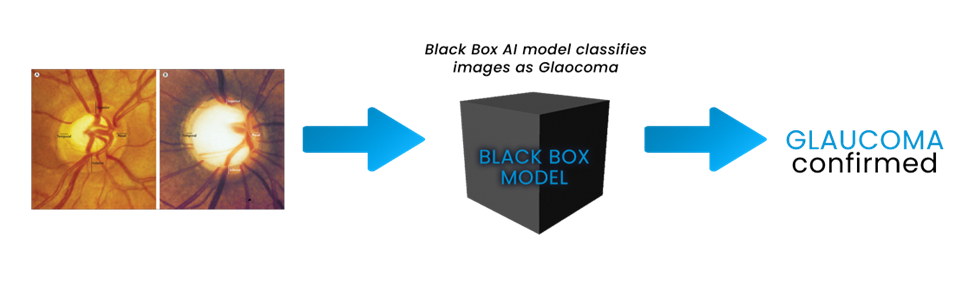
\includegraphics[scale=0.70]{images/fig-1.png}
\caption{Blackbox models confirming glaucoma through images}
\label{fig:x Blackbox models confirming glaucoma through images}
\end{figure}

\vspace{5mm}
In Figure 4.2 we will see how black boxes actually work with the help of lime.

\vspace{5mm}
\begin{figure}[htbp]
\centering
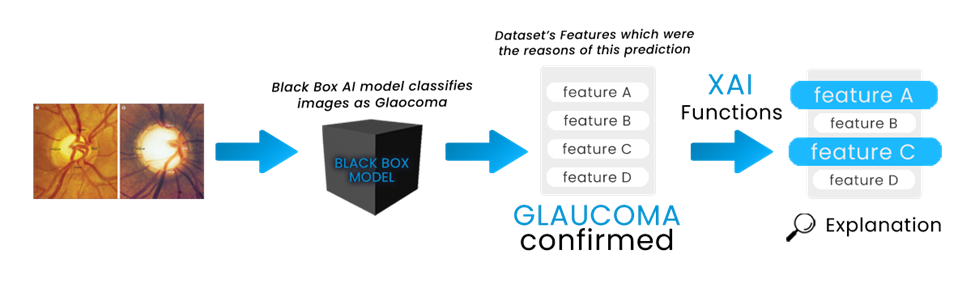
\includegraphics[scale=0.70]{images/fig-2.png}
\caption{Blackbox models decision making explanation through LIME}
\label{fig:x Blackbox models decision making explanation through LIME}
\end{figure}

\vspace{5mm}
Here we can see BlackBox models generate a result or output based on some features from the given/training datasets. And through lime, we can have a visualization from which features the output was based on.

\vspace{5mm}
In our Glaucoma dataset, we have some features for Suspicious glaucoma and Non-glaucoma. In both sections, we have \textbf{attention map}, \textbf{images}, and \textbf{labels} as \textbf{1} as the confirmed glaucoma case and \textbf{0} as the Non-glaucoma case. To apply XAI, we took \textbf{Convolutional Neural Network (CNN)}, \textbf{Support Vector Machine (SVM)}, \textbf{Fully Connected Neural Network (FCNNs)} as a black box AI model to predict glaucoma with the help of the data. To compile all of these classifications and determine the average of these scores to one single output, we will use the Softmax function. Below a short rendition is being given for the above Deep Learning models.

\vspace{5mm}
1.    \textbf{Convolutional Neural Network (CNN)}: In deep learning, a convolutional neural network (CNN, or ConvNet) is a class of deep neural networks, most commonly applied to analyze visual imagery. We will classify the image data through this model.

\vspace{5mm}
2.    \textbf{Support Vector Machine (SVM)}: SVM is a supervised machine learning classifier that may be used to categorize or to regression problems.
It uses a method called the kernel trick to transform your data and then calculates an appropriate boundary between various outputs based on these modifications. With this model, we will get a predicted output.

\vspace{5mm}
3.    \textbf{Fully Connected Neural Network (FCNNs)}: Fully connected neural networks (FCNNs) are a type of artificial neural network where the architecture is such that all the nodes, or neurons, are in one layer, are connected to the neurons in the next layer [22]. This model will also help us to predict and output.

\vspace{5mm}
4.    \textbf{Softmax}: Softmax is a mathematical function that transforms a vector of integers into a vector of probabilities, with the probability of each value proportional to the vector's relative scale. The softmax function is most commonly used as an activation function in a neural network model in applied machine learning. The network is set up to produce N values, one for each classification task class, and the softmax function is used to normalize the outputs, turning them from weighted sum values to probabilities that total to one. Each value in the output of the softmax function is interpreted as the probability of membership for each class. This will compile the outputs of SVM and FCNNs into a single output.

\newpage
\section{Work Plan} 
According to our Dataset, we will divide the data in a ratio of 8:2 chronologically training and testing data to classify glaucoma with the help above deep learning models. And through any XAI function, we will explain these black boxes.

\begin{figure}[htbp]
\centering
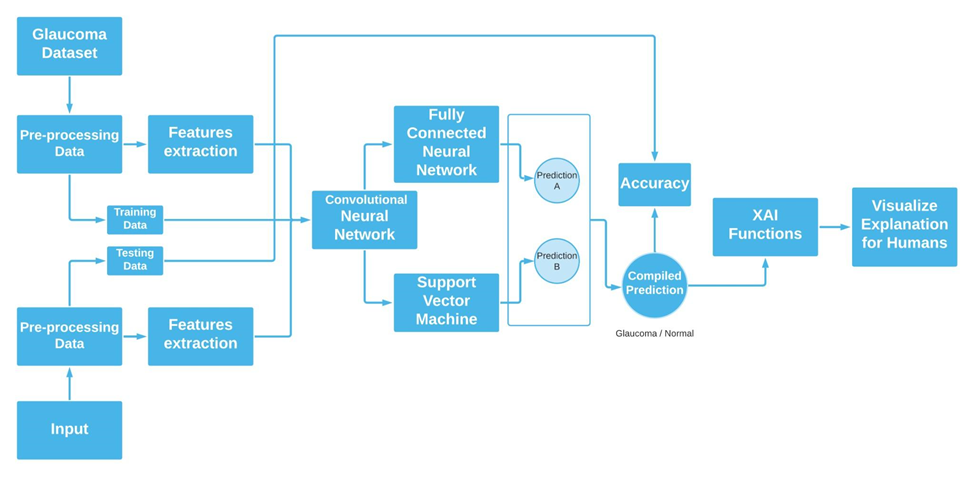
\includegraphics[scale=0.75]{images/fig-3.png}
\caption{Work plan of the whole project}
\label{fig:x Work plan of the whole project}
\end{figure}

\vspace{5mm}
Here in [Figure 4.3], we have shown the whole process from dataset preprocessing to compiled output through Softmax. And with XAI functions, we will explain the black boxes through visualization charts of the used core features which were the main reasons behind the prediction.

\chapter{Implementation}
%\section{Implementation}
\section{Fundamentals of Deep Learning}

Deep learning is a type of machine learning and artificial intelligence (AI) that imitates the way humans gain certain types of knowledge. While traditional machine learning algorithms are linear, deep learning algorithms are stacked in a hierarchy of increasing complexity and abstraction [23].

\vspace{5mm}
\noindent Neural Networks are basically made-up of several units which work mimicking the human brain's neurons. Each neuron is connected to another one in order to generate a particular problem to solve. These neurons in AI are called units.

\vspace{5mm}
\noindent The input layer is the very first neuron of an Artificial brain. It takes raw data from the dataset and passes it to the next-level neurons. And the layer which produces the final output is called the output layer. These input and output layers may contain N number of units. Output layers units may depend on the output layer classes. In-between these two layers, there can be N numbers of hidden layers, each containing its own weights and biases so that it can calculate its next neuron's journey. The given weight of the connection is multiplied to its corresponding input and then added up resulting in a weighted sum, on which the activation function implies and produces the activation for that neuron, which is indeed the output of the neuron denoted by y. Then, an activation function will get triggered as an output for this y.

\vspace{5mm}
\begin{figure}[hbt!]
\centering
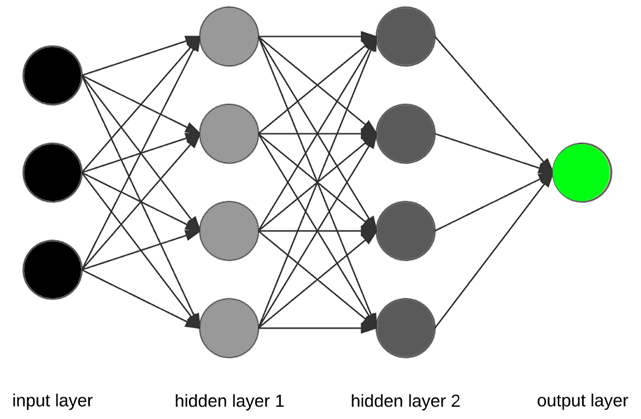
\includegraphics[scale=0.3]{images/fig-4.png}
\caption{Hidden Layer Between Input and Output Layers}
\label{fig:x Hidden Layer Between Input and Output Layers}
\end{figure}

\section{Dataset, Libraries, and Tools}
As our data are mostly direct fundus images from LAG-Dataset[24]. CNN is being used in this thesis for image classification, as it is a type of model which processes data such as images. Also, it automatically understands low-to high-level patterns of image classification. which helps us to extract higher representations for the image content.

\vspace{5mm}
\begin{figure}[htbp]
\centering
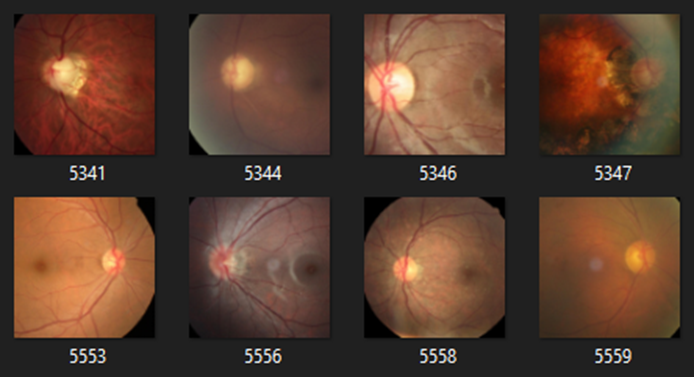
\includegraphics[scale=1]{images/fig-5.png}
\caption{Sample Data form LAG-Dataset}
\label{fig:x Sample Data form LAG-Dataset}
\end{figure}

\noindent This dataset contains 4250 images for \textbf{training}, 302 images for testing and 302 images for \textbf{validation}. All of these folders have two folders for glaucoma and non-glaucoma. The label for “glaucoma” is 1 and for “non-glaucoma” is 0.

\vspace{5mm}
\begin{table}[htbp]
\centering
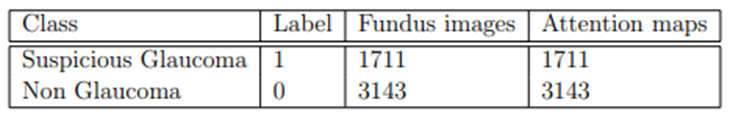
\includegraphics[scale=1]{images/fig-6.png}
\caption{\label{tab:Distribution of data with labels}Distribution of data with labels}

% \label{fig:x Distribution of data with labels }
\end{table}

\noindent In this study, we are going to use the \textbf{python} programming language. It is a high level OOP programming language that has a lot of amazing Machine learning libraries.

\vspace{5mm}
\noindent For this research we are using :

\begin{itemize}
    \item IDE (Google Colab & Jupyter Notebook)
    \item GPU (GTX 1660 super OC)
\end{itemize}

\newpage
\noindent Some of the Libraries that we are going to use are :

\vspace{5mm}
\noindent \textbf{TensorFlow}: TensorFlow is an end-to-end open-source platform for machine learning. It has a comprehensive, flexible ecosystem of tools, libraries, and communities [17].

\vspace{5mm}
\noindent \textbf{Keras}: Keras is the high-level API of TensorFlow 2: an approachable, highly-productive interface for solving machine learning problems [18]

\vspace{5mm}
\noindent \textbf{Matplotlib}: Matplotlib is a comprehensive library for creating static, animated, and interactive visualizations in Python.[25]

\vspace{5mm}
\noindent \textbf{Pandas}: Pandas is an open-source, BSD-licensed library providing high-performance, easy-to-use data structures, and data analysis tools for Python programming [26]

\vspace{5mm}
\noindent \textbf{Numpy}: NumPy offers comprehensive mathematical functions, random number generators, linear algebra routines, Fourier transforms, and more [19]

\vspace{5mm}
\noindent \textbf{Scikit-Learning}: Simple and efficient tools for predictive data analysis · Accessible to everybody, and reusable in various contexts · Built on NumPy, SciPy, and matplotlib [27]
 
\section{Architecture of the Proposed Model}
In deep learning, a convolutional neural network (CNN, or ConvNet) is a class of artificial neural networks, most commonly applied to analyze visual imagery[20].

\vspace{5mm}
\noindent In this study, a Transfer Learning approach is proposed. The data set's size and features provide a perfect environment for implementing a transfer learning approach, allowing a pre-trained CNN with all of its weights to be utilized to develop a new transfer learning model specialized to identifying Glaucoma with a high degree of accuracy.

\vspace{5mm}
\begin{figure}[hbt!]
\centering
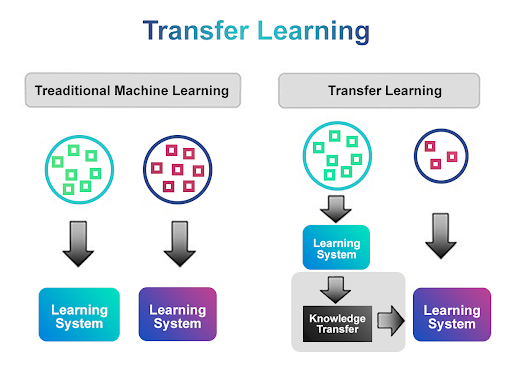
\includegraphics[scale=0.75]{images/fig-7.png}
\caption{Sample Data form LAG-Dataset}
\label{fig:x Sample Data form LAG-Dataset}
\end{figure}

\vspace{5mm}
\noindent We are going with the Fine-Tuning approach of Transfer Learning.

\vspace{5mm}
\noindent The CNN Models we are using are:

\begin{itemize}
    \item VGG-16
    \item InceptionV3
    \item VGG-19
    \item ResNet50
    \item DenseNet121
\end{itemize}

\subsection{VGG-16}
With 16-19 layers of weights and small convolution filters of (33), the VGG[29] Convolutional Neural Network built by Visual Geometry Group, the University of Oxford has achieved amazing results. ReLU non-linearly is used here for hidden layers.

\vspace{5mm}
\noindent Here, we used the Keras implementation of the VGG16 model. We used the weights learned from the ImageNet dataset. We didn’t use the 3 fully connected layers at the top of the network. Input shape of the images is 224 x 224 and there are 3 channels. First, we flattened the model outputs. We used the “ReLU” activation function for the layers. For predictions, we used the “Softmax” activation function. 

\vspace{5mm}
\noindent In figure 5.4 we can visualize the architecture of the VGG-16  model.

\vspace{5mm}
\begin{figure}[hbt!]
\centering
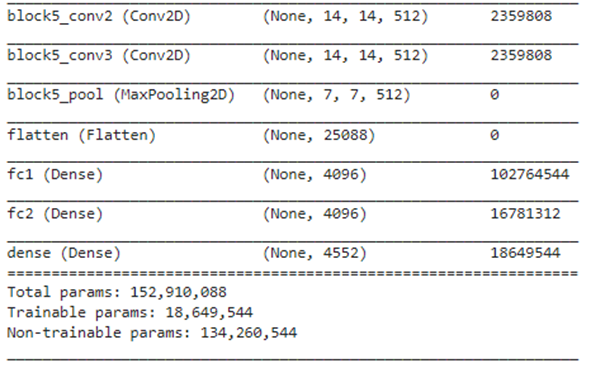
\includegraphics[scale=0.5]{images/fig-8.png}
\caption{Model Summary of VGG-16}
\label{fig:x Model Summary of VGG-16}
\end{figure}

\vspace{5mm}
\noindent In figure 5.5 we can visualize the architecture of the VGG-16  model.

\vspace{5mm}
\begin{figure}[hbt!]
\centering
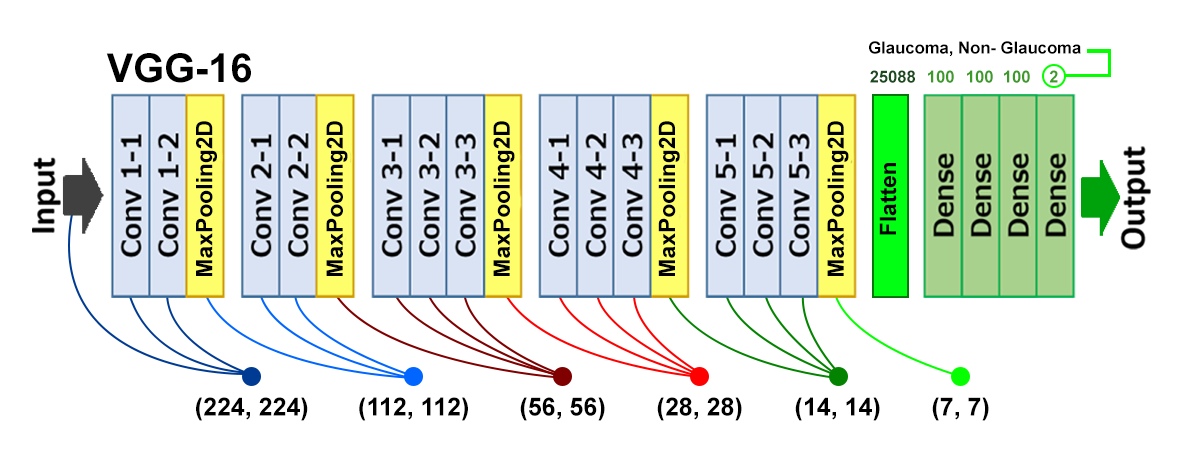
\includegraphics[scale=0.75]{images/Architecture of VGG-16.png}
\caption{Architecture of VGG-16}
\label{fig:x Architecture of VGG-16}
\end{figure}

\subsection{Inception V3}
The Inception [30] architecture is made up of several inception modules stacked on top of each other to form a deep neural network, where the inception modules provide the ability to operate them all in parallel and concatenate their outputs into a single output vector for input to the module afterward. 

\vspace{5mm}
\noindent Here we used Keras implementation of inceptionV3 model. We used the weights learned from the ImageNet dataset. We didn’t use the 3 fully connected layers at the top of the network. Input shape of the images is 224 x 224 and there are 3 channels. First, we flattened the model outputs. We used the “ReLU” activation function for the layers. For predictions, we used the “Softmax” activation function.

\vspace{5mm}
\begin{figure}[hbt!]
\centering
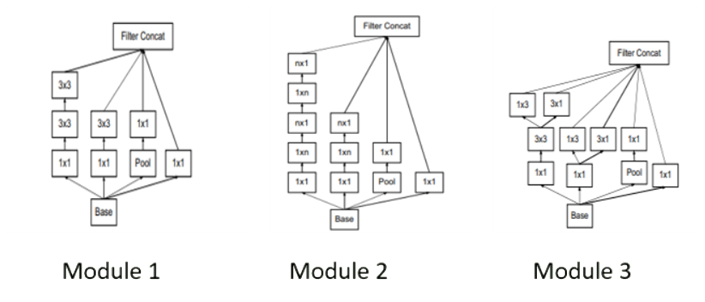
\includegraphics[scale=0.5]{images/fig-10.png}
\caption{The three inception modules}
\label{fig:x The three inception modules}
\end{figure}

\vspace{5mm}
\noindent In our proposed transfer learning model, we use InceptionV3, a new form of the inception architecture. Table 5.2 depicts the InceptionV3 network architecture. Each module's output size is the next module's input size. 

\begin{table}[hbt!]
\centering
\begin{tabular}{|c | c | c|}
\hline
Type & patch size & input size\\
\hline
conv & 3 x 3/2 & 224 x 224 x 3\\
\hline
conv & 3 x 3/1 & 149 x 149 x 32\\
\hline
conv padded & 3x3 / 1 & 147 x 147 x 32\\
\hline
pool & 3x3/2 & 147 x 147 x 64\\
\hline
conv & 3×3/1 & 73 × 73 × 64\\
\hline
conv & 3×3/2 & 71 × 71 × 80\\
\hline
conv & 3×3/1 & 35 × 35 × 192\\
\hline
3×Inception & module 1 & 35 × 35 × 288\\
\hline
5×Inception & module 2 & 17 × 17 × 768\\
\hline
2×Inception & module 3 & 8 × 8 × 1280\\
\hline
pool & 8×8 & 8 ×8 × 2048\\
\hline
linear & logits & 1 ×1 × 2048\\
\hline
softmax & classifier & 1 ×1 × 1000\\
\hline

\end{tabular}
\caption{Outline of the InceptionV3 architecture}
\label{tab:Outline of the InceptionV3 architecture [31]
)}
\end{table}

\noindent In figure 5.7 we can visualize our model summary of InceptionV3.

\vspace{5mm}
\begin{figure}[hbt!]
\centering
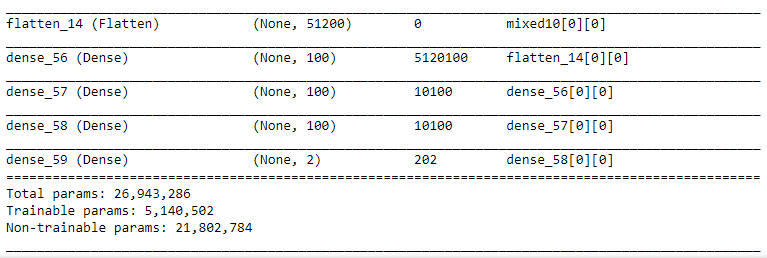
\includegraphics[scale=0.75]{images/fig-11.png}
\caption{Model Summary of InceptionV3}
\label{fig:x Model Summary of InceptionV3}
\end{figure}

\subsection{VGG-19}
VGG19 is a variant of the VGG model which in short consists of 19 layers (16 convolution layers, 3 fully connected layers, 5 MaxPool layers, and 1 SoftMax layer). [32] VGG19 has 19.6 billion Flops.

\vspace{5mm}
\noindent Here, we used the Keras implementation of the VGG19 model. We used the weights learned from the ImageNet dataset. We didn’t use the 3 fully connected layers at the top of the network. Input shape of the images is 224 x 224 and there are 3 channels. First, we flattened the model outputs. Then we performed batch normalization. We used a dropout rate of 0.5. We used the “ReLU” activation function for the layers.

\vspace{5mm}
\noindent For predictions, we used the “Softmax” activation function. For the Gradient Descent, we used the Adam optimizer with a learning rate of \(10^-5\). In Figure 5.8, Our model summary for VGG-19 is given.

\vspace{5mm}
\begin{figure}[hbt!]
\centering
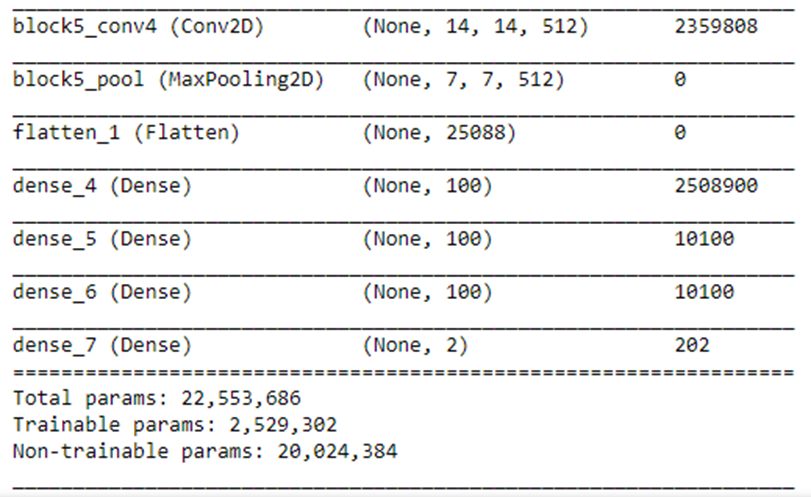
\includegraphics[scale=1]{images/fig-12.png}
\caption{Model Summary of VGG-19}
\label{fig:x Model Summary of VGG-19}
\end{figure}

\vspace{5mm}
\begin{figure}[hbt!]
\centering
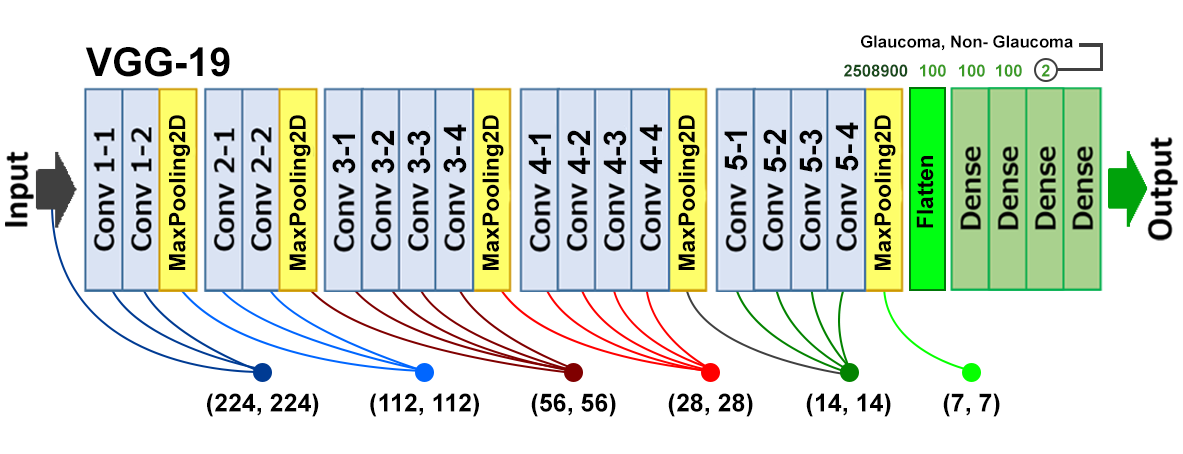
\includegraphics[scale=0.75]{images/Architecture of VGG-19.png}
\caption{Architecture of VGG-19}
\label{fig:x Architecture of VGG-19}
\end{figure}

\subsection{ResNet50}
ResNet50 is a version of the ResNet model which has 48 convolution layers and 1 MaxPool layer and 1 average pool layer. Moreover, it has 3.8 x \(10^9\) floating-point operations. ResNet50 plays an important role in the computer vision and deep learning world. It is mainly used for image recognition and is most commonly applied for analyzing visual imagery. Also, it is a pre-trained Deep Learning model for image classification of the Convolutional Neural Network (CNN). ResNet50 is mainly trained on a million images of 1000 categories from the ImageNet database and there are over 23 million trained parameters which will make it more suitable for image recognition. ResNet50 is deeper than any other network using residual connections.

\vspace{5mm}
\noindent Here, we used the Keras implementation of the ResNet50 Model. We used the weights learned from the ImageNet dataset. We didn’t use the 3 fully connected layers at the top of the network. Input shape of the images is 224 x 224 and there are 3 channels. First, we flattened the model outputs. Then we performed batch normalization. We used a dropout rate of 0.5. We used the “ReLU” activation function for the layers. Again we performed batch normalization and used a dropout rate of 0.5. For predictions, we used the “Softmax” activation function. 

\vspace{5mm}
\begin{figure}[hbt!]
\centering
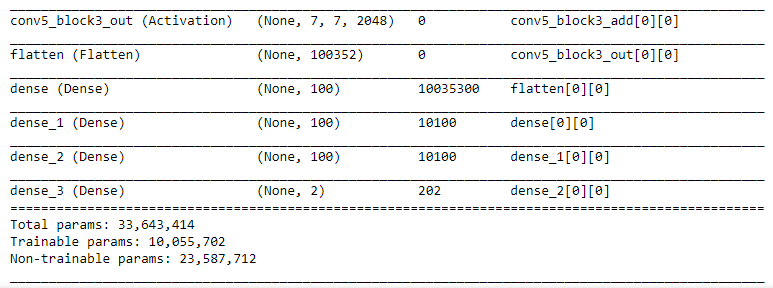
\includegraphics[scale=0.75]{images/ResNet50.PNG}
\caption{Model Summary of ResNet50}
\label{fig:x Model Summary of ResNet50}
\end{figure}

\subsection{DenseNet121}
Dense Convolutional Network which is DenseNet is an architecture that spotlights on making the profound learning networks go considerably more profound, and yet making them more proficient to prepare, by utilizing more limited associations between the layers [33]. DenseNet is very much like ResNet for certain key distinctions. For instance, ResNet utilizes an added substance strategy that combines the preceding layer with the future layer, while DenseNet links the result of the preceding layer with the future layer. This is done to empower the greatest data stream between the layers of the organization.

\vspace{5mm}
\noindent Here, we used the Keras implementation of the DenseNet121 model . We used the weights learned from the ImageNet dataset. We didn’t use the 3 fully connected layers at the top of the network. Input shape of the images is 224 x 224 and there are 3 channels. We performed  the 2D Global Average Pooling. Then we performed batch normalization. We used a dropout rate of 0.5. We used the “ReLU” activation function for the layers and again performed batch normalization and used a dropout rate of 0.5. For predictions, we used the “Softmax” activation function.

\vspace{5mm}
\begin{figure}[hbt!]
\centering
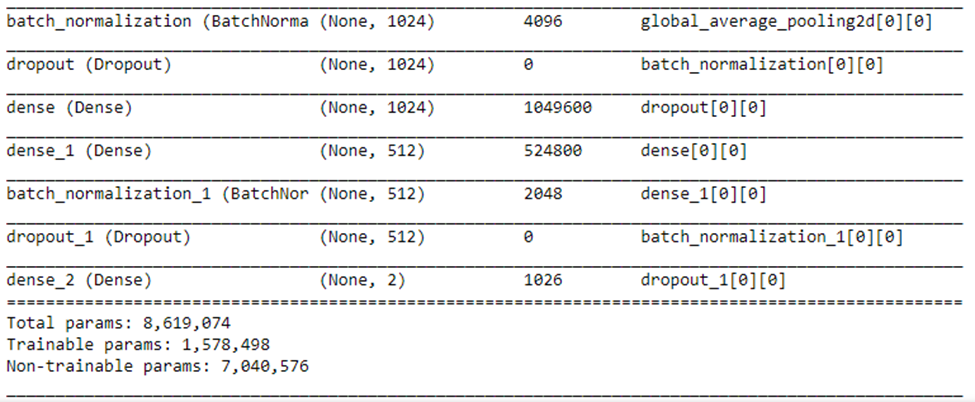
\includegraphics[scale=0.5]{images/fig-15.png}
\caption{Model Summary of DenseNet121}
\label{fig:x Model Summary of DenseNet121}
\end{figure}

\section{Fine Turing}
Fine-tuning is the process of fine-tuning or changing a model that has already been trained for one task to make it execute a second related task. A deep learning network that recognizes cars, for example, maybe fine-tuned to recognize trucks [25]. As proposed, we will be using Fine-tuning approach to detect Glaucoma from our dataset which will help to detect our wanted result in this study

\vspace{5mm}
\begin{figure}[hbt!]
\centering
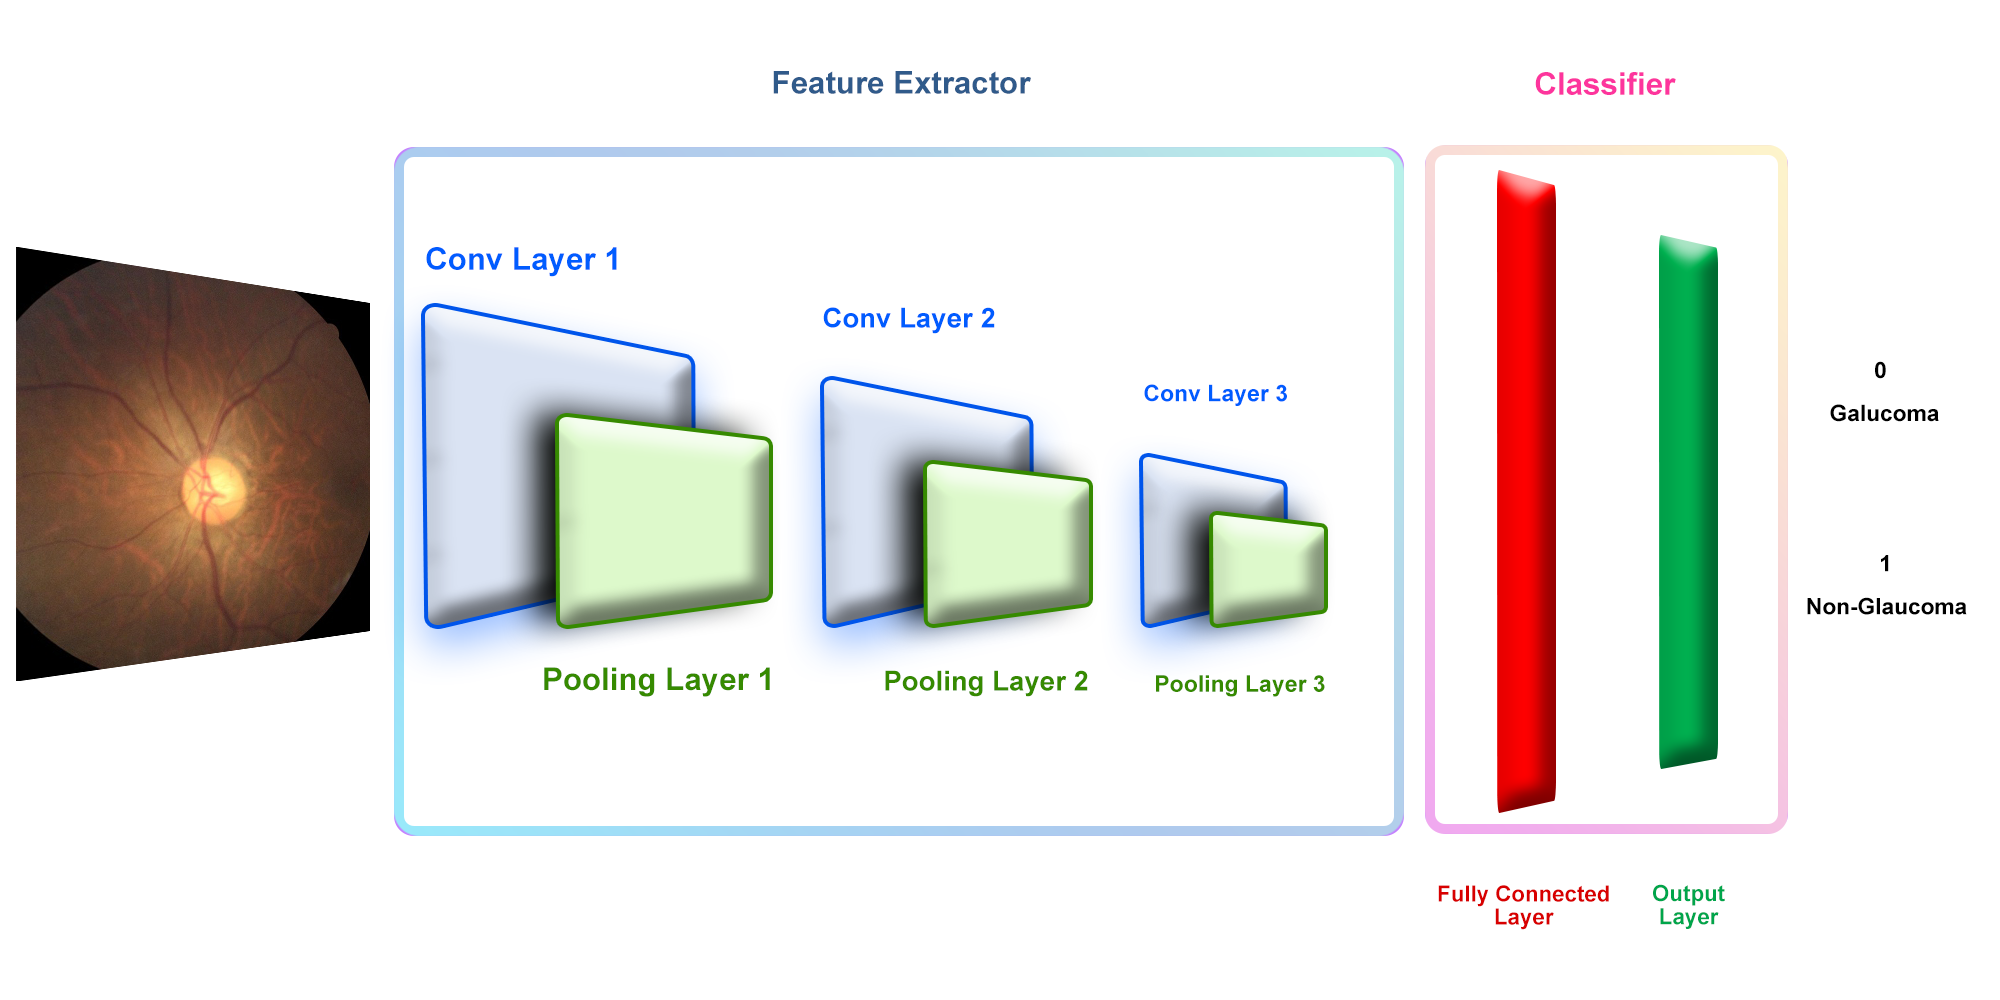
\includegraphics[scale=0.4]{images/Fine-tuning by keeping the feature extractor_s final layers trainable.png}
\caption{Fine-tuning by keeping the feature extractor's final layers trainable}
\label{fig:x Fine-tuning by keeping the feature extractor's final layers trainable}
\end{figure}

\newpage
\subsection{Segments of CNN}

\vspace{5mm}
The architecture of Convolutional Neural Networks is basically 3 types of layers.

\begin{itemize}
    \item Convolutional
    \item Pooling
    \item Fully Connected
\end{itemize}

\vspace{5mm}
\begin{figure}[hbt!]
\centering
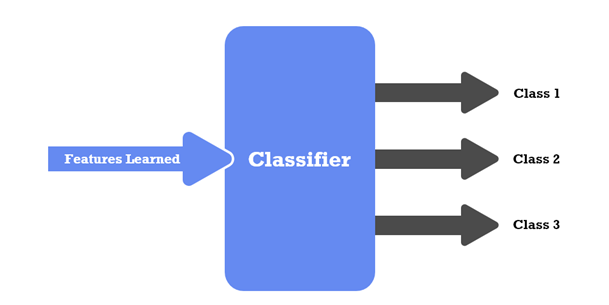
\includegraphics[scale=1]{images/fig-17.png}
\caption{CNN Classifier}
\label{fig:x CNN Classifier}
\end{figure}

\noindent And basically, all these layers do these operations as bellow:

\vspace{5mm}
\begin{itemize}
    \item Convolution operation
    \item Pooling operation
    \item Flattening
    \item Non-linear activation functions imply
    \item Optimization operation
\end{itemize}

\vspace{5mm}
\subsection{Convolutional Operation}


\vspace{5mm}
The convolutional layers, which are the fundamental building blocks of CNN, are responsible for convolution operations and produce feature maps that learn the features of the image taken as input by convolving appropriately learned filters or kernels with the input array or tensor, as shown in \textbf{figure 5.14}. A convolution layer, as shown in \textbf{figure 5.15}, has a number of feature maps that record new features and respond to feature hierarchy throughout the neural network, from the early layers to the distant edging layers.[29][34][30]

\newpage
\vspace{5mm}
\begin{figure}[hbt!]
\centering
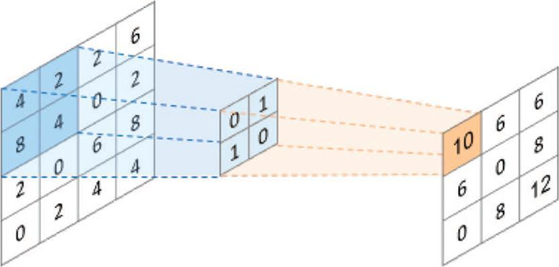
\includegraphics[scale=1]{images/fig-18.png}
\caption{On the input tensor, a kernel is applied, resulting in a feature map}
\label{fig:x On the input tensor, a kernel is applied, resulting in a feature map}
\end{figure}

\vspace{5mm}
\begin{figure}[hbt!]
\centering
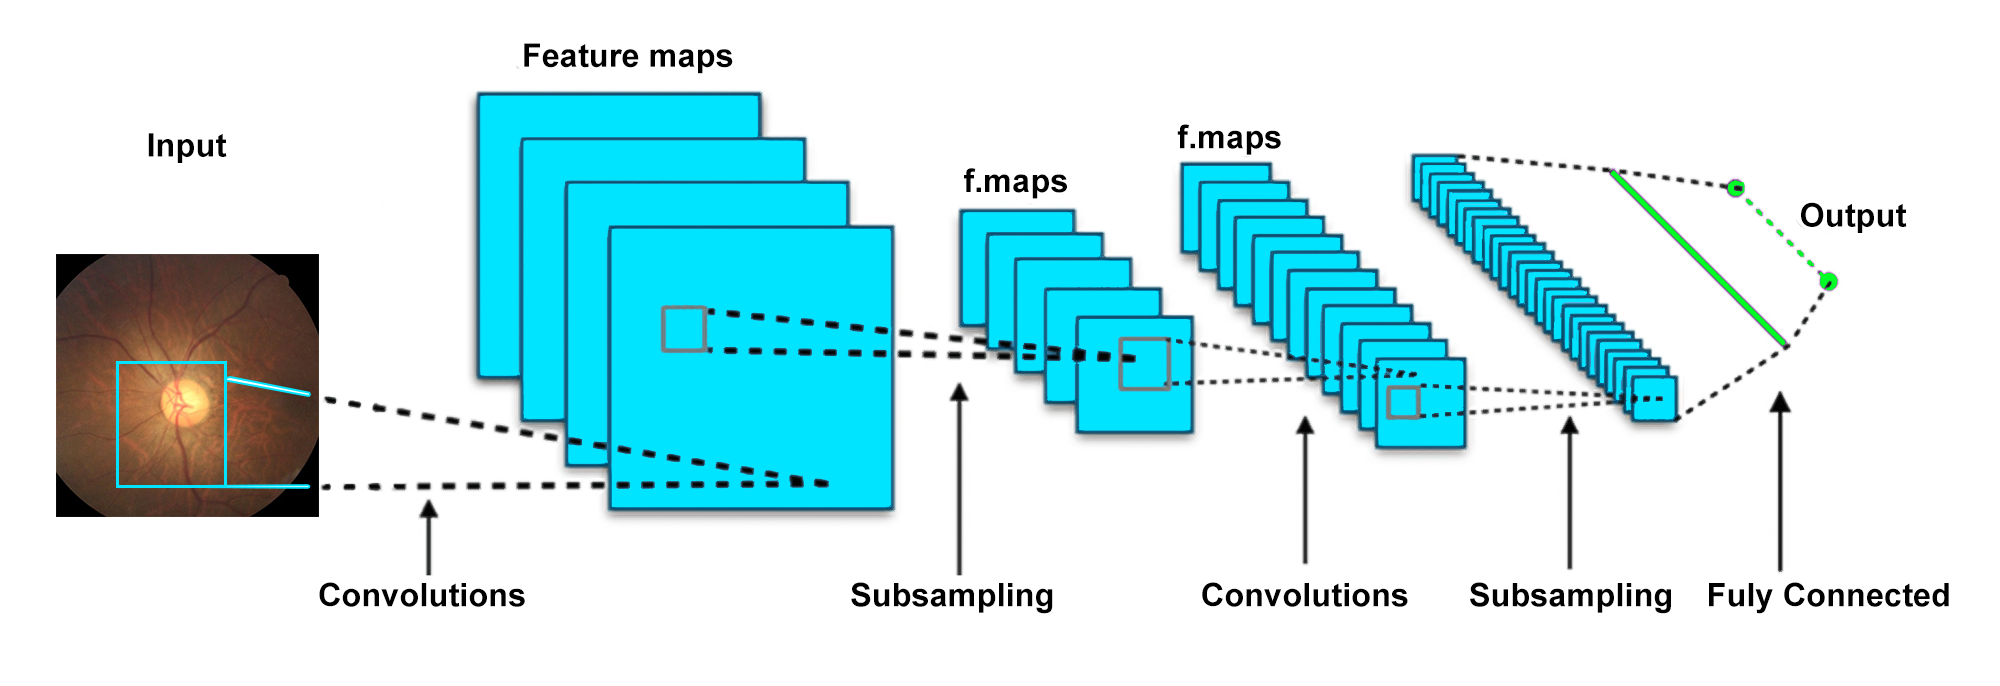
\includegraphics[scale=0.4]{images/planes shown are a feature map.png}
\caption{Planes shown are a feature map}
\label{fig:x Planes shown are a feature map}
\end{figure}

\subsection{Pooling Operation}

\vspace{5mm}
The feature maps are pooled in order to extract more features and minimize their dimension[30]. In general, the pooling operation is carried out as follows:

\vspace{5mm}
\begin{figure}[hbt!]
\centering
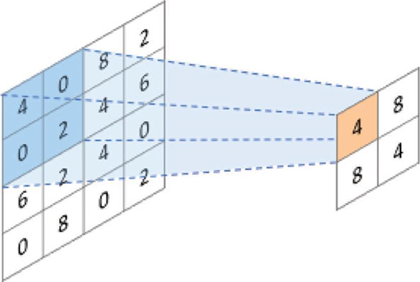
\includegraphics[scale=1]{images/fig-20.png}
\caption{Pooling Operation}
\label{fig:x Pooling Operation}
\end{figure}

\vspace{5mm}
\begin{itemize}
    \item \textbf{Max Pooling}: The maximum value of a patch of numbers from the feature map used as input is returned as an output. [30]
    \item \textbf{Average Pooling}: It produces the average value of a patch of numbers from the feature map that was used as input as an output. [34]
    \item \textbf{GlobalAveragePooling2D}:GlobalAveragePooling2D does something different. It applies average pooling on the spatial dimensions until each spatial dimension is one.
\end{itemize}

\vspace{5mm}
\begin{figure}[hbt!]
\centering
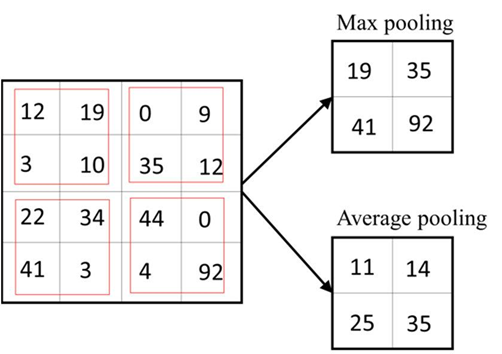
\includegraphics[scale=1]{images/fig-21.png}
\caption{Max and Average Pooling}
\label{fig:x Max and Average Pooling}
\end{figure}

\vspace{5mm}
\subsection{Flattening Layers}

\vspace{5mm}
Flattening is the process of turning data into a one-dimensional array for use in the following layer. To produce a single lengthy feature vector, we flatten the output of the convolutional layers. It's also linked to the final classification model, which is referred to as a fully-connected layer. [35]

\vspace{5mm}
\begin{figure}[hbt!]
\centering
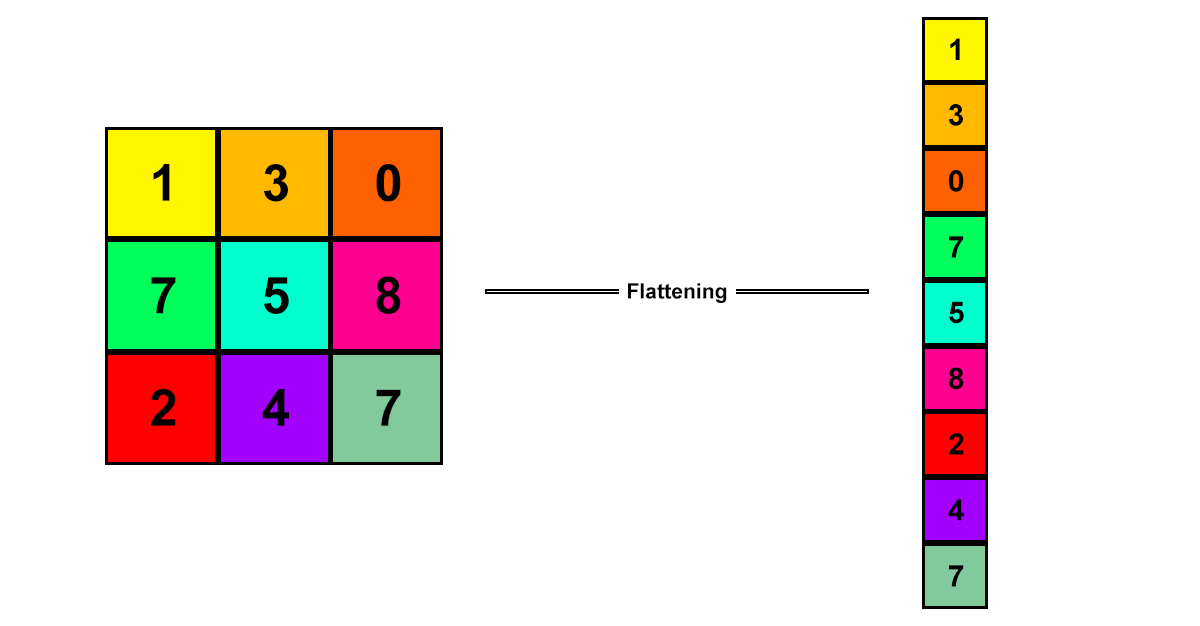
\includegraphics[scale=0.5]{images/Pooling Matrix to Flattening..png}
\caption{Pooling Matrix to Flattening.}
\label{fig:x Pooling Matrix to Flattening}
\end{figure}

\vspace{5mm}
\subsection{Fully Connected Layers}

\vspace{5mm}
In a neural network, fully connected layers are those where all of the inputs from one layer are connected to every activation unit of the subsequent layer. The last few layers in most standard machine learning models are fully connected layers that assemble the data collected by subsequent layers to produce the final output.[36]

\vspace{5mm}
\begin{figure}[hbt!]
\centering
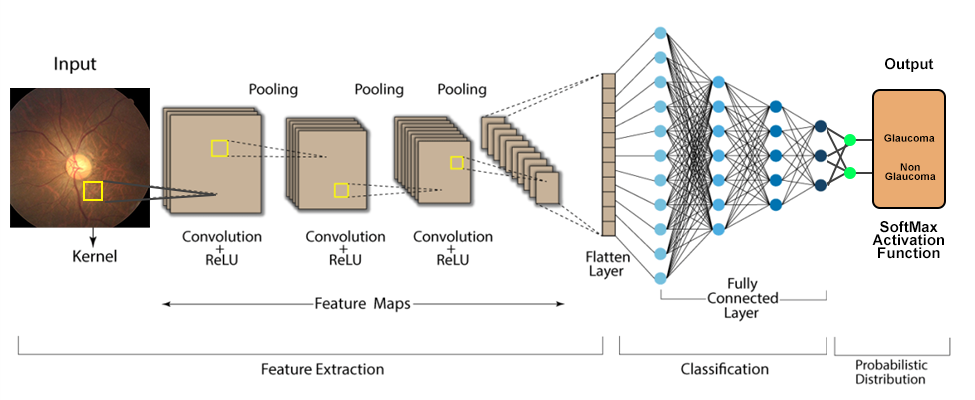
\includegraphics[scale=0.45]{images/Fully Connected CNN classifying between classes.png}
\caption{Fully Connected CNN classifying between classes}
\label{fig:x Fully Connected CNN classifying between classes}
\end{figure}

\noindent Fully connected layers or in other words dense layers take nonlinear activation functions, however, the final output layer of the fully connected layers take Softmax activation.

\vspace{5mm}
\noindent We are also going to use sigmoid and ReLU in both VGG-16 and InceptionV3.

\vspace{5mm}
\subsection{Batch Normalization}

\vspace{5mm}
While feeding input to Neural Networks, we do Batch Normalization because it makes the training faster and handles internal covariate shift. Again Normalizing the input for a similar range of values can speed up the learning. Because Batch Normalization normalizes the outputs of the activation functions in every layer of the neural network, not just in the inputs. In their original paper, Sergey et al. [37] claim that Batch Normalization reduces the internal covariate shift of the network.

\vspace{5mm}
\subsection{Dropout}

\vspace{5mm}
Adulteration of training information misleadingly regulates to overfit through dropout and other characteristical noise systems. Dropout holds out a kind of versatile regularization for summed up straight models [38]. Moreover, Dropout is a normal stochastic choice strategy in view of the neural organization [39]. This has the effect of making the layer look and be treated as a layer with a particular measure of hubs and availability to the past layer. Essentially, a particular perspective on the designed layer is directed with each update to a layer during preparing.

\section{Analysis}
We have used VGG-16, VGG-19, DenseNet121, InceptionV3 and ResNet50 models for our study. Every model was compiled with Adam optimizer with the learning rate of 1e-5 in 50 epochs. 

\noindent These are the score(validation accuracy) our models - 

\vspace{5mm}
\begin{figure}[hbt!]
\centering
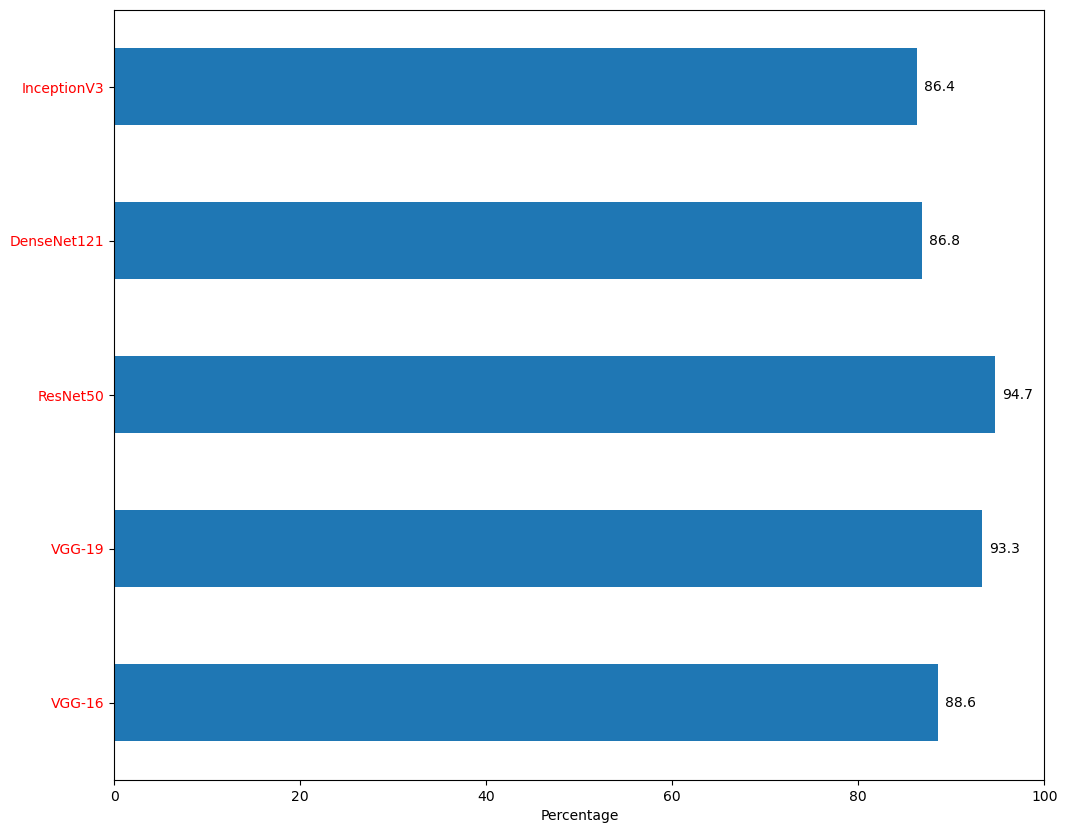
\includegraphics[scale=0.5]{images/fig-24.png}
\caption{Fully Connected CNN classifying between classes}
\label{fig:x Fully Connected CNN classifying between classes.}
\end{figure}

\noindent After 50 epochs, RestNet50 got the highest score among the other models with a validation accuracy of 94.7\%.

\vspace{5mm}
\noindent These are the Train and Test accuracy and loss graph for each model.

\newpage
\vspace{5mm}
\noindent Model Accuracy and Loss of VGG-16 -

\vspace{5mm}
\begin{figure}[hbt!]
\centering
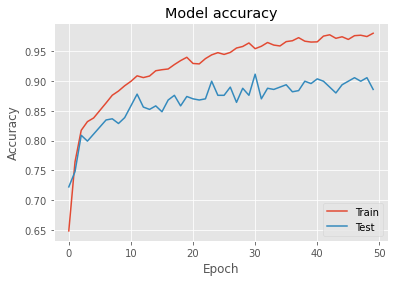
\includegraphics[scale=1]{images/fig-25.png}
\caption{VGG-16 Model Train and Test Accuracy}
\label{fig:x VGG-16 Model Train and Test Accuracy}
\end{figure}

\vspace{5mm}
\begin{figure}[hbt!]
\centering
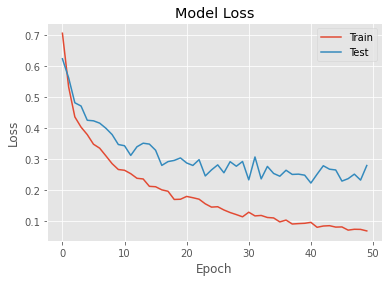
\includegraphics[scale=1]{images/fig-26.png}
\caption{VGG-16 Model Train and Test Loss}
\label{fig:x VGG-16 Model Train and Test Loss}
\end{figure}

\newpage
\noindent Model Accuracy and Loss of VGG-19 -

\vspace{5mm}
\begin{figure}[hbt!]
\centering
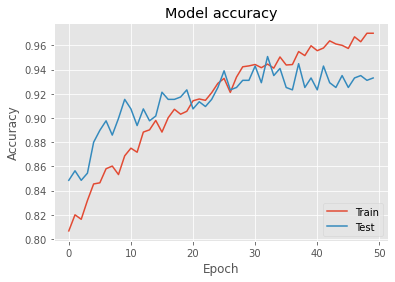
\includegraphics[scale=1]{images/fig-27.png}
\caption{VGG-19 Model Train and Test Accuracy}
\label{fig:x VGG-19 Model Train and Test Accuracy}
\end{figure}

\vspace{5mm}
\begin{figure}[hbt!]
\centering
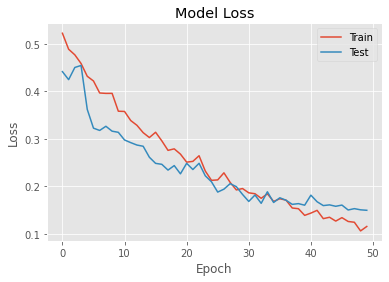
\includegraphics[scale=1]{images/fig-28.png}
\caption{VGG-19 Model Train and Test Loss}
\label{fig:x VGG-19 Model Train and Test Loss}
\end{figure}

\newpage
\vspace{5mm}
\noindent Model Accuracy and Loss of ResNet50 -
\vspace{5mm}
\begin{figure}[hbt!]
\centering
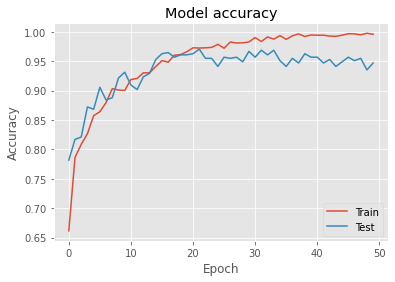
\includegraphics[scale=1]{images/fig-29.png}
\caption{ResNet50 Model Train and Test Accuracy}
\label{fig:x ResNet50 Model Train and Test Accuracy}
\end{figure}

\vspace{5mm}
\begin{figure}[hbt!]
\centering
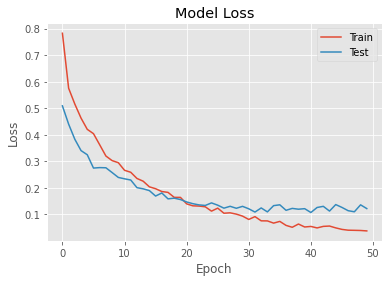
\includegraphics[scale=1]{images/fig-30.png}
\caption{ResNet50 Model Train and Test Loss}
\label{fig:x ResNet50 Model Train and Test Loss}
\end{figure}

\newpage
\vspace{5mm}
\noindent Model Accuracy and Loss of DenseNet121 -
\vspace{5mm}
\begin{figure}[hbt!]
\centering
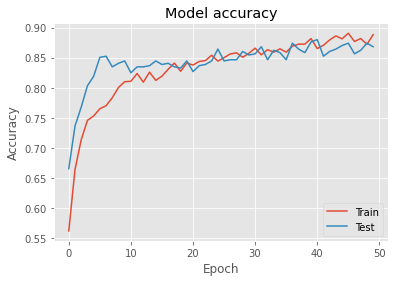
\includegraphics[scale=1]{images/fig-31.png}
\caption{DenseNet121 Model Train and Test Accuracy}
\label{fig:x DenseNet121 Model Train and Test Accuracy}
\end{figure}

\vspace{5mm}
\begin{figure}[hbt!]
\centering
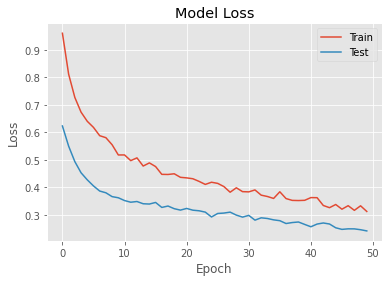
\includegraphics[scale=1]{images/fig-32.png}
\caption{DenseNet121 Model Train and Test Loss}
\label{fig:x DenseNet121 Model Train and Test Loss}
\end{figure}

\newpage
\vspace{5mm}
\noindent Model Accuracy and Loss of InceptionV3 -
\vspace{5mm}
\begin{figure}[hbt!]
\centering
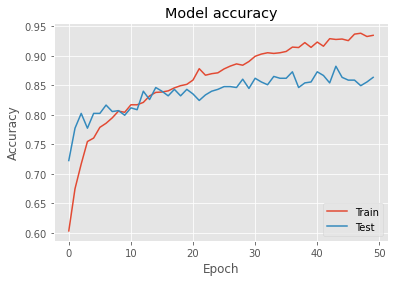
\includegraphics[scale=1]{images/fig-33.png}
\caption{InceptionV3 Model Train and Test Accuracy}
\label{fig:x InceptionV3 Model Train and Test Accuracy}
\end{figure}

\vspace{5mm}
\begin{figure}[hbt!]
\centering
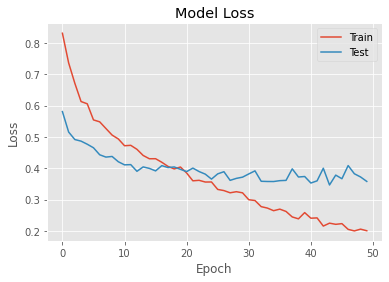
\includegraphics[scale=1]{images/fig-34.png}
\caption{InceptionV3 Model Train and Test Loss}
\label{fig:x InceptionV3 Model Train and Test Loss}
\end{figure}

\noindent The shape and dynamics of a learning curve can be used to diagnose the behavior of a machine learning model and in turn perhaps suggest the type of configuration changes that may be made to improve learning and/or performance.

\vspace{5mm}
\noindent There are three common dynamics that you are likely to observe in learning curves. And they are:

\begin{itemize}
    \item Underfit
    \item Overfit
    \item Good Fit
\end{itemize}

\noindent We know that smaller relative scores on the y-axis indicate more or better learning. 

\vspace{5mm}
\begin{figure}[hbt!]
\centering
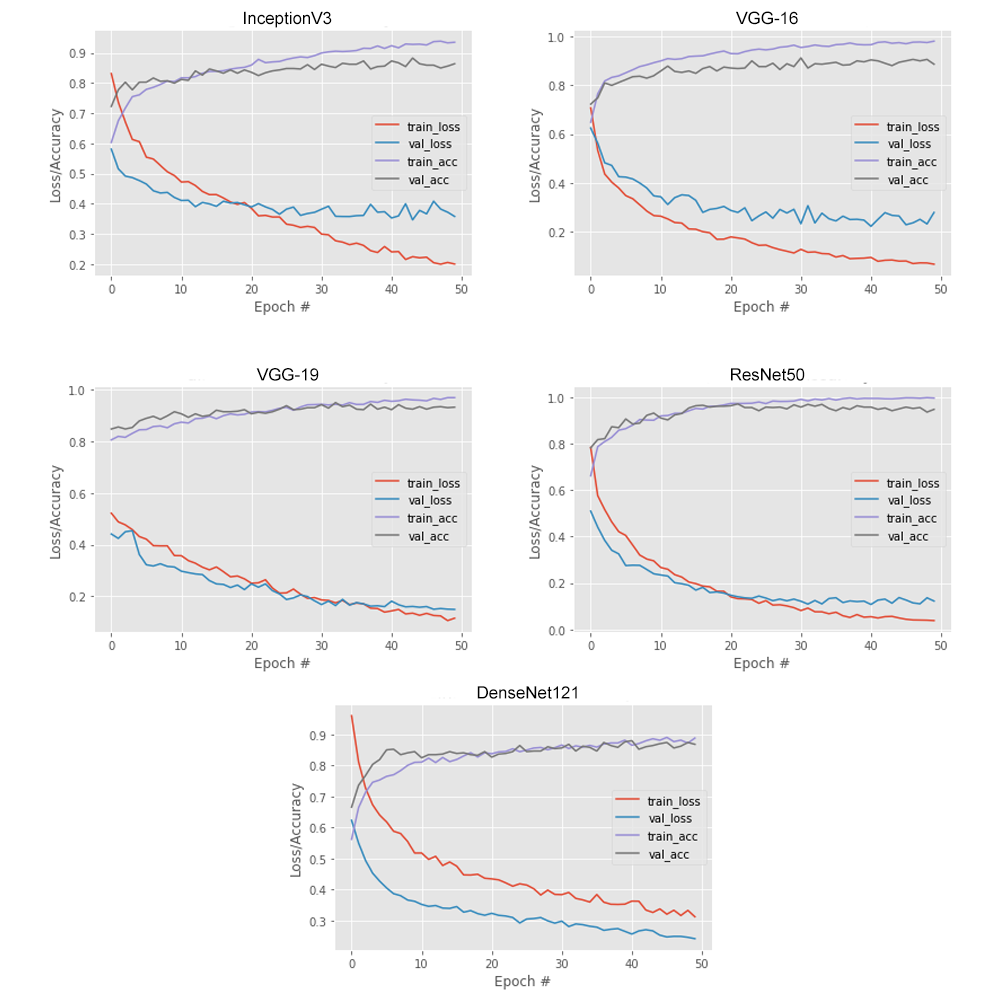
\includegraphics[scale=0.75]{images/fig-35.png}
\caption{All Model’s Train Test Accuracy and Loss Curve}
\label{fig:x All Model’s Train Test Accuracy and Loss Curve}
\end{figure}

\vspace{5mm}
\noindent Comparing All models' Accuracy and Loss graph together, we can see that VGG-19 and ResNet50 were the Good-Fit than the other models.

\vspace{5mm}
\noindent These are the Train sets, True and Predicted scores of classified and misclassified glaucoma and non-glaucoma results for each model based on the model’s train datasets prediction labels and the actual train labels. We have added a threshold of 0.5 for this train predicted visualization.

\vspace{5mm}
\noindent (the percentages are meaning the predicted train accuracy for the predicted labels calculated with the actual train labels)

\vspace{5mm}
\begin{figure}[hbt!]
\centering
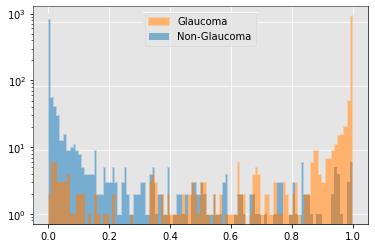
\includegraphics[scale=0.75]{images/fig-36.png}
\caption{True and Predicted Train scores of DenseNet121}
\label{fig:x True and Predicted Train scores of DenseNet121}
\end{figure}

% \centering
\begin{center}
All  151 misclassified samples (93.83\%) 

Glaucoma  74 misclassified samples (93.95\%)

Non-Glaucoma  77 misclassified samples (93.71\%)
\end{center}
\vspace{5mm}
\begin{figure}[hbt!]
\centering
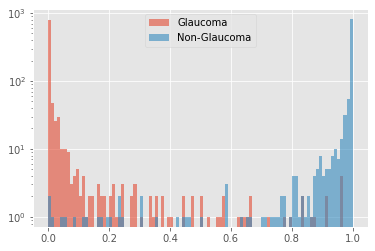
\includegraphics[scale=0.75]{images/fig-37.png}
\caption{True and Predicted Train scores of InceptionV3}
\label{fig:x True and Predicted Train scores of InceptionV3}
\end{figure}

% \centering
\begin{center}
All   48 misclassified samples (97.65\%)

Glaucoma  22 misclassified samples (97.84\%)

Non-Glaucoma  26 misclassified samples (97.45\%)
\end{center}
\vspace{5mm}
\begin{figure}[hbt!]
\centering
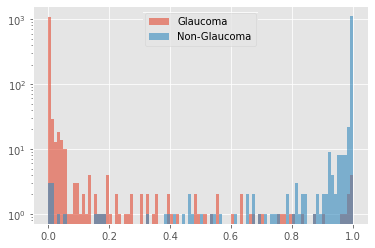
\includegraphics[scale=0.75]{images/fig-38.png}
\caption{True and Predicted Train scores of VGG-16}
\label{fig:x True and Predicted Train scores of VGG-16}
\end{figure}

\newpage
% \centering
\begin{center}
All   47 misclassified samples (98.08\%)

Glaucoma  20 misclassified samples (98.37\%)

Non-Glaucoma  27 misclassified samples (97.79\%)
\end{center}
\vspace{5mm}
\begin{figure}[hbt!]
\centering
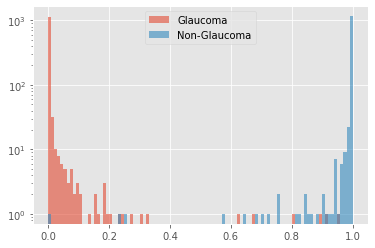
\includegraphics[scale=0.75]{images/fig-39.png}
\caption{True and Predicted Train scores of VGG-19}
\label{fig:x True and Predicted Train scores of VGG-19}
\end{figure}
\begin{center}
All   17 misclassified samples (99.31\%)

Glaucoma  14 misclassified samples (98.86\%)

Non-Glaucoma   3 misclassified samples (99.75\%)
\end{center}
\vspace{5mm}
\begin{figure}[hbt!]
\centering
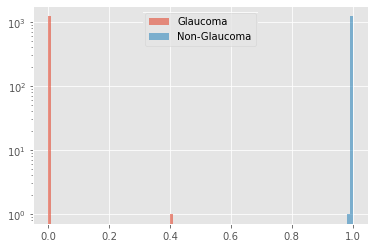
\includegraphics[scale=0.75]{images/fig-40.png}
\caption{True and Predicted Train scores of ResNet50}
\label{fig:x True and Predicted Train scores of ResNet50}
\end{figure}

\newpage
\begin{center}
All    0 misclassified samples (100.00\%)

Glaucoma   0 misclassified samples (100.00\%)

Non-Glaucoma   0 misclassified samples (100.00\%)
\end{center}
\vspace{5mm}
Now, We have called the same function that we have used for the above Train predicted labels again with the same threshold of 0.5. But for now we have used the validation datasets prediction labels. And the results were - 

\noindent \textit{(the percentages are meaning the predicted test/validation accuracy for the predicted labels calculated with the actual test/validation labels)}

\noindent \textit{( Here, G = Glaucoma and n-G = Non-Glaucoma )}

\begin{center}
\begin{table}[hbt!]
\centering
\begin{tabular}{|p{3cm}|p{3cm}|p{3cm}|c|}\toprule
\hline
% \parbox{\centering \textbf{Model}} & \parbox{\centering \textbf{All misclassified}} & \parbox{\centering \textbf{G misclassified}} & \parbox{\centering \textbf{n-G misclassified}} \\

\centering{\textbf{Model} & \centering\textbf{All misclassified} & \centering\textbf{G misclassified} & \textbf{n-G misclassified}} \\
\hline
\centering DenseNet121 & \centering 9 (86.76\%) & \centering 4 (88.24\%) & 5 (85.29\%)\\
\hline
\centering InceptionV3 & \centering 24 (85.88\%) & \centering 16 (81.18\%) & 8 (90.59\%)\\
\hline
\centering VGG-16 & \centering 8 (88.24\%) & \centering 7 (79.41\%) & 1 (97.06\%)\\
\hline
\centering VGG-19 & \centering 4 (94.12\%) & \centering 3 (91.18\%) & 1 (97.06\%)\\
\hline
\centering ResNet50 & \centering 3 (95.59\%) & \centering 1 (97.06\%) & 2 (94.12\%)\\
\hline
\bottomrule
\end{tabular}
\caption{True and Predicted Test scores of all Model}
\label{tab:True and Predicted Test scores of all Model}
\end{table}
\end{center}



\vspace{5mm}
\noindent Now we have taken a single predicted batch from each model’s prediction with the 0.5 threshold and plotted the misclassified glaucoma and non-glaucoma images, which we will use in Lime (XAI framework) to explain later.

\noindent \textit{( Here, G = Glaucoma and n-G = Non-Glaucoma )}
\begin{center}
\begin{table}[hbt!]
\centering
\begin{tabular}{|c | c | c| c |}
\hline
\textbf{Model} & \textbf{Batch} & \textbf{G misclassified} & \textbf{n-G misclassified}}\\

\hline
DenseNet121 & 2 (32 in each) & 3 &  5\\
\hline
InceptionV3 & 2 (32 in each) & 2 & 7\\
\hline
VGG-16 & 2 (32 in each) & 2 & 3\\
\hline
VGG-19 & 2 (32 in each) & 1 & 4\\
\hline
ResNet50 & 2 (32 in each) & 0 & 3\\
\hline

\end{tabular}
\caption{True and Predicted Test scores of all Model}
\label{tab:True and Predicted Test scores of all Model}
\end{table}
\end{center}
\newpage
\vspace{5mm}
\noindent These are some of the misclassified images for all models with and undoing the existing preprocessing. Basically the model’s preprocessing for these images ruined their actual color and contrast.  Which led the model to predict wrong. By undoing the existing preprocessing we can see that for DesneNet121 the images got a little reddish and for other models, It got bluish.

\vspace{5mm}
\begin{figure}[hbt!]
\centering
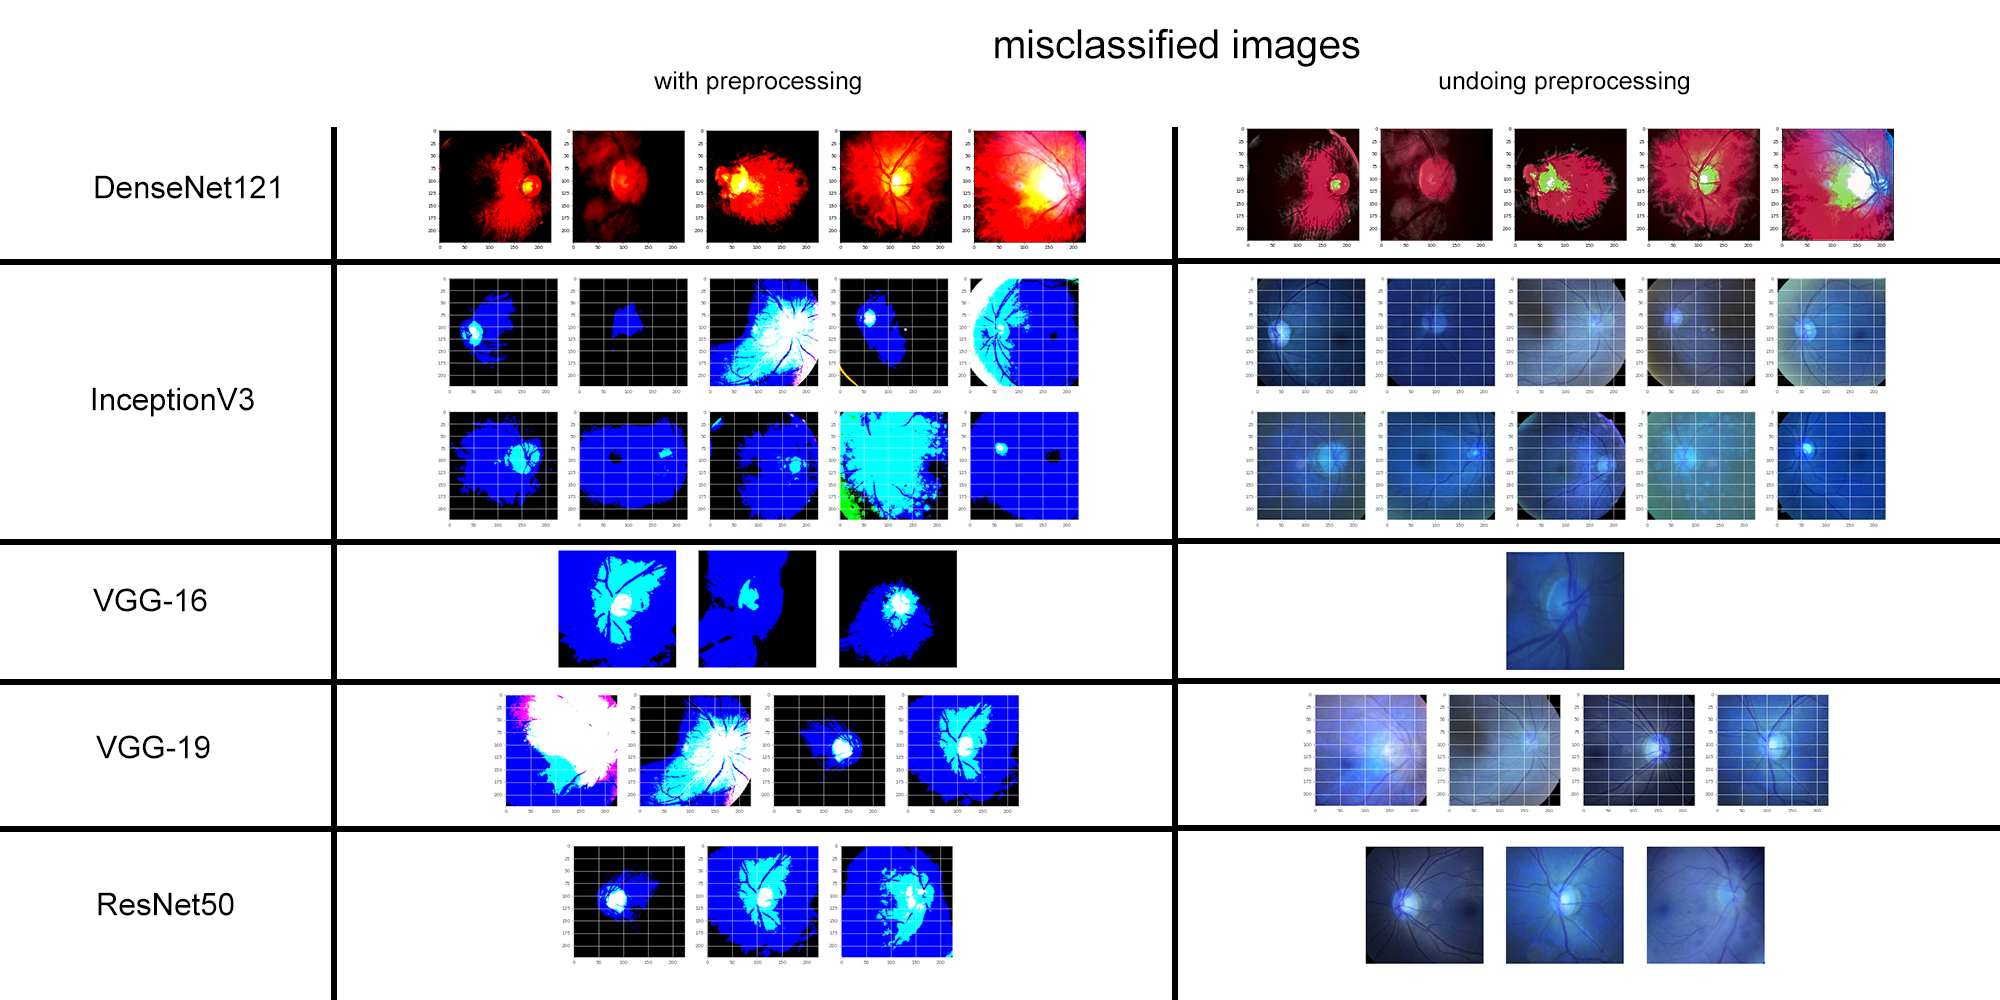
\includegraphics[scale=0.42]{images/fig-41.png}
\caption{Misclassified images for all models with and without preprocessing}
\label{fig:x True and Predicted Train scores of ResNet50}
\end{figure}

\vspace{5mm}
\noindent Now we will show the explanation for these preprocessed and misclassified images using an XAI[40] framework, \textbf{LIME}. Then we will apply Lime again on a single predicted raw fundus -image directly from the test dataset (labelled) directory to see the difference between a correctly predicted fundus image[42] and wrong predicted fundus image.
Given below are the the misclassified image with preprocessing, Superpixels focused area and the model prediction explanation by Lime in DenseNet121

\vspace{5mm}
\begin{figure}[hbt!]
\centering
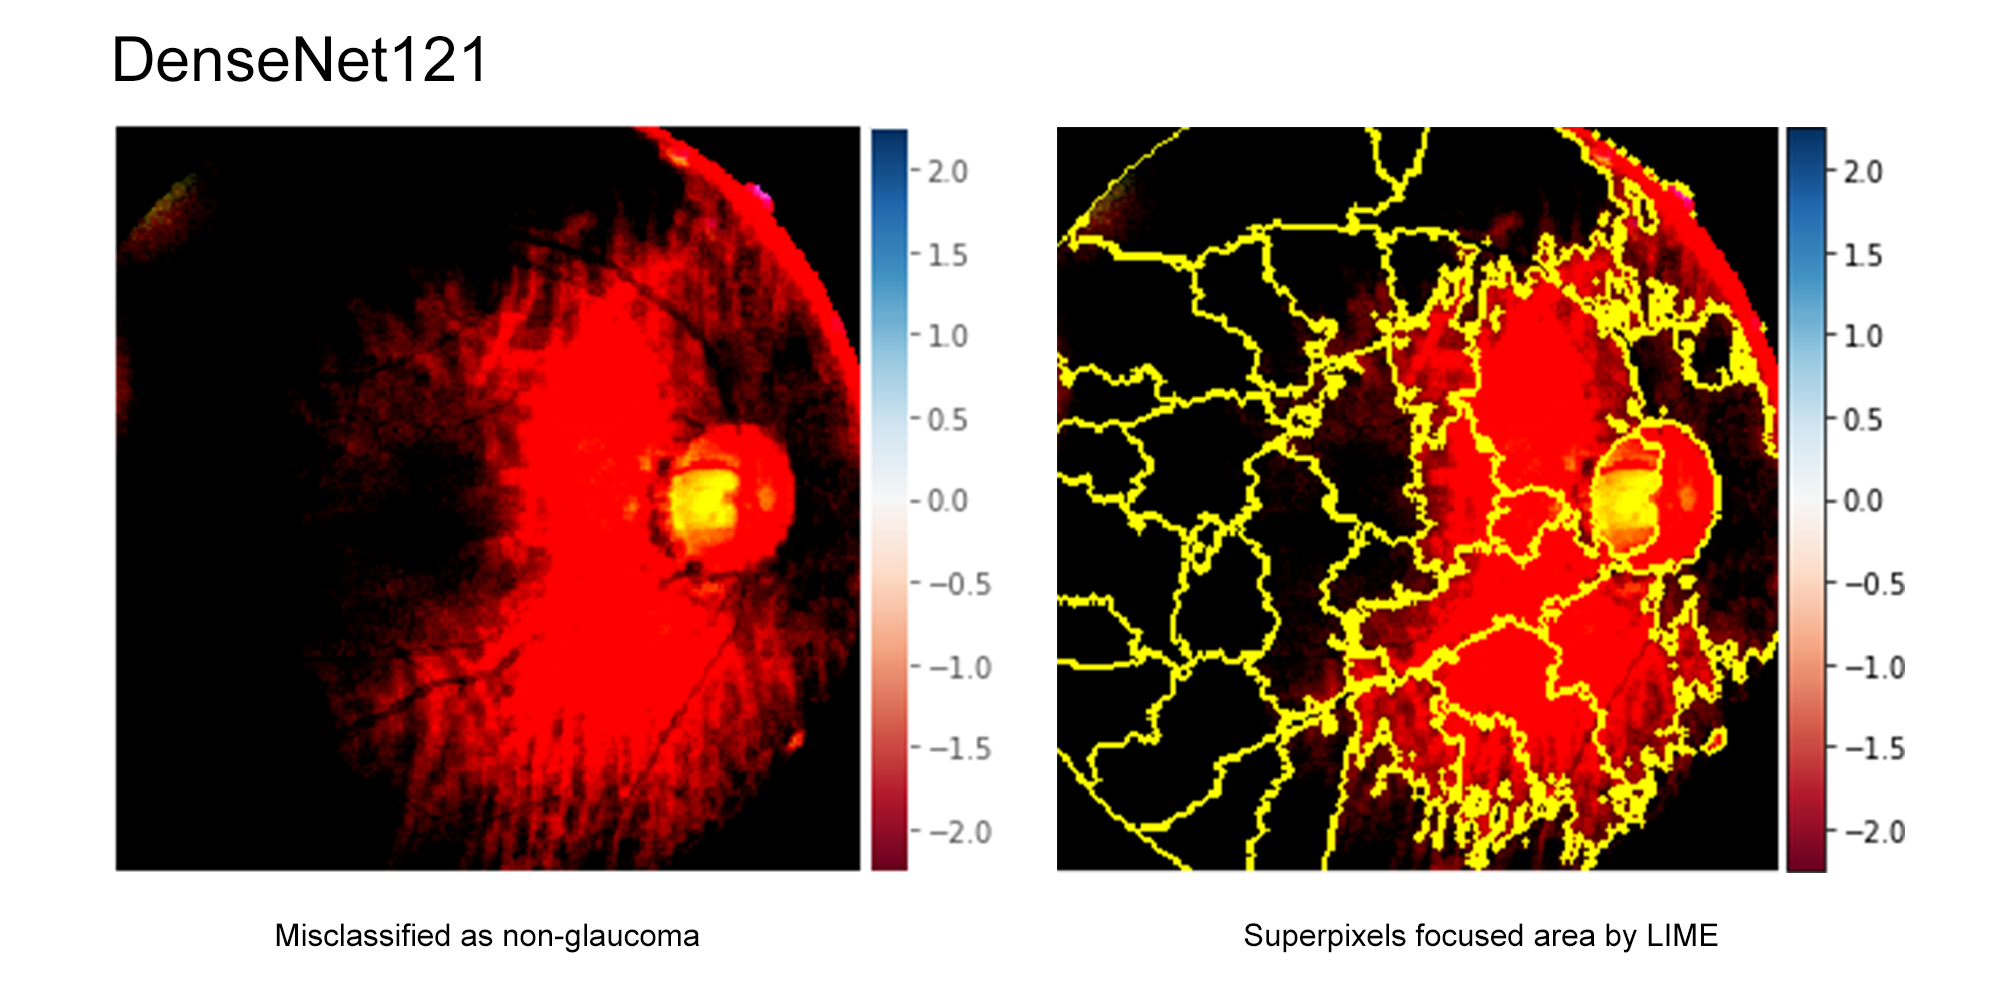
\includegraphics[scale=0.45]{images/fig-42.png}
\caption{Misclassified image with preprocessing and Superpixels focused area by Lime in DenseNet121}
\label{fig:x Misclassified image with preprocessing and Superpixels focused area by Lime in DenseNet121}
\end{figure}

\vspace{5mm}
\begin{figure}[hbt!]
\centering
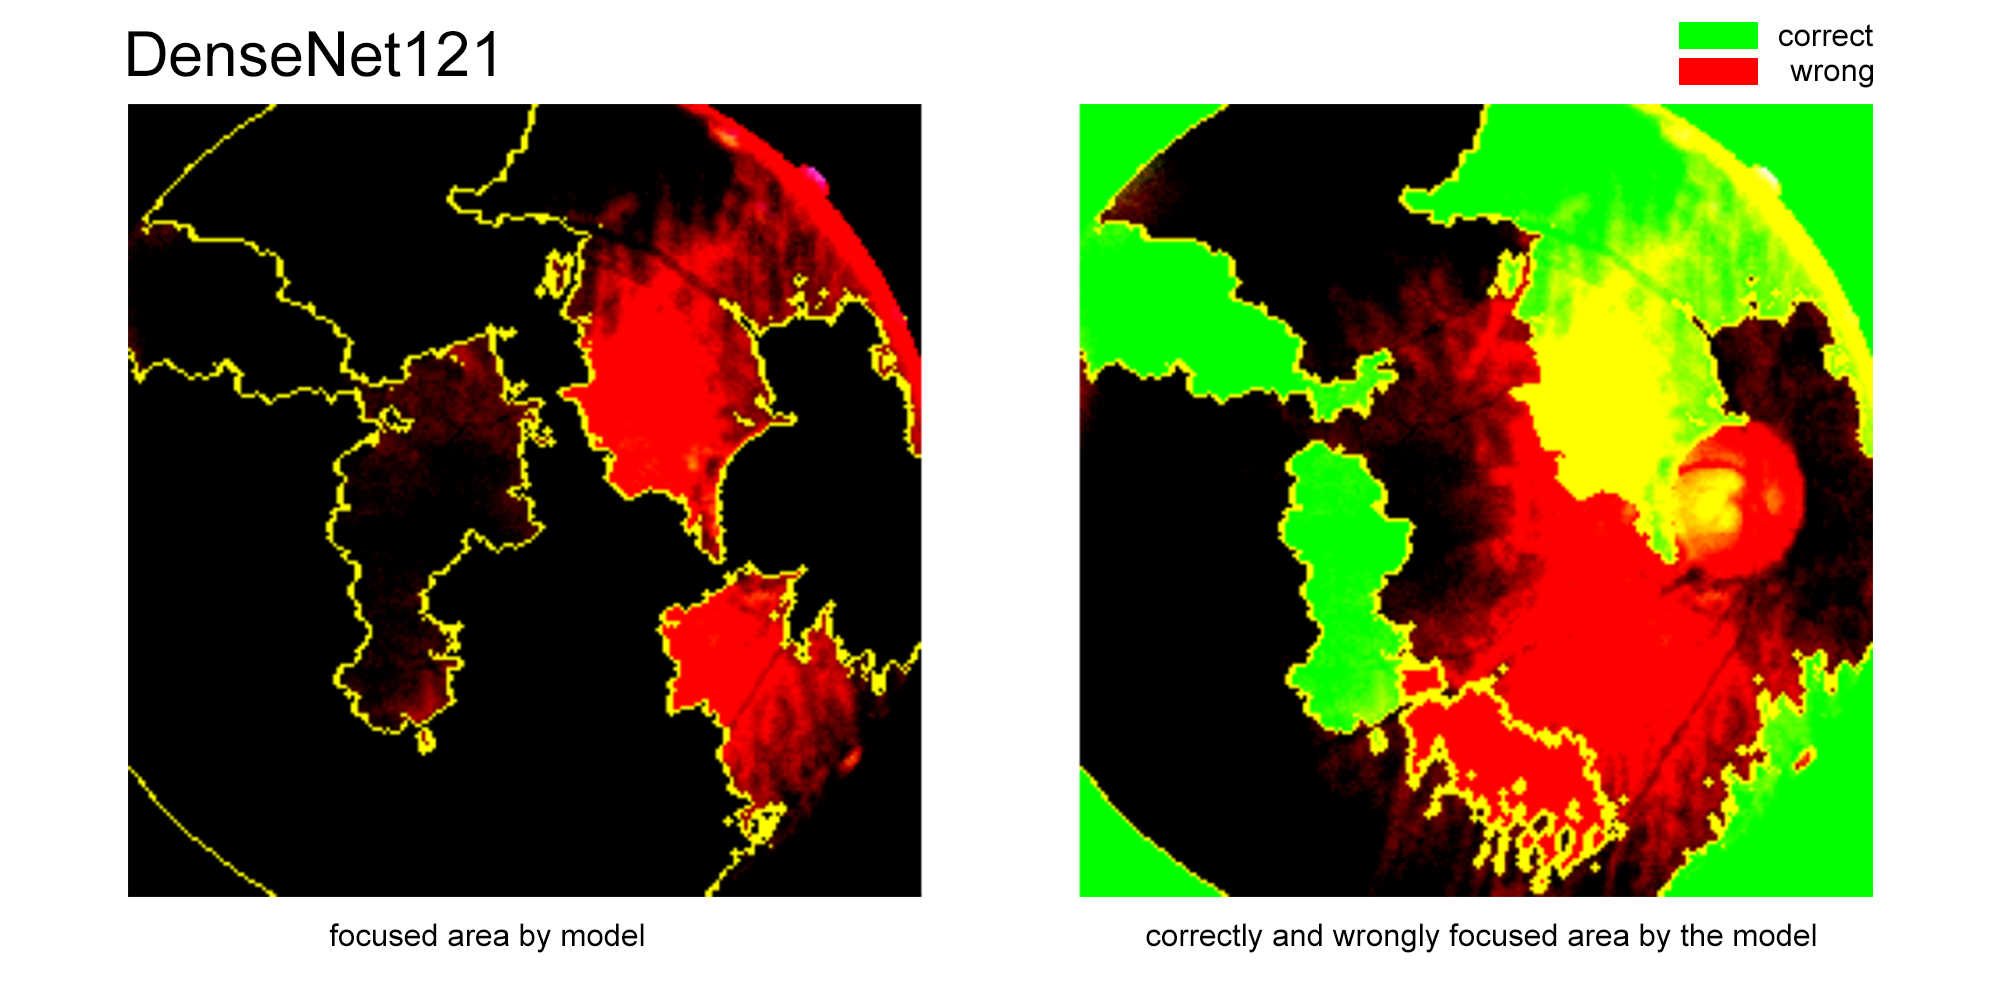
\includegraphics[scale=0.45]{images/fig-43.png}
\caption{Lime Explanation for DenseNet121}
\label{fig:x Lime Explanation for DenseNet121}
\end{figure}

\newpage
\vspace{5mm}
\noindent Given below are the the misclassified image with preprocessing, Superpixels focused area and the model prediction explanation by Lime in InceptionV3 -

\vspace{5mm}
\begin{figure}[hbt!]
\centering
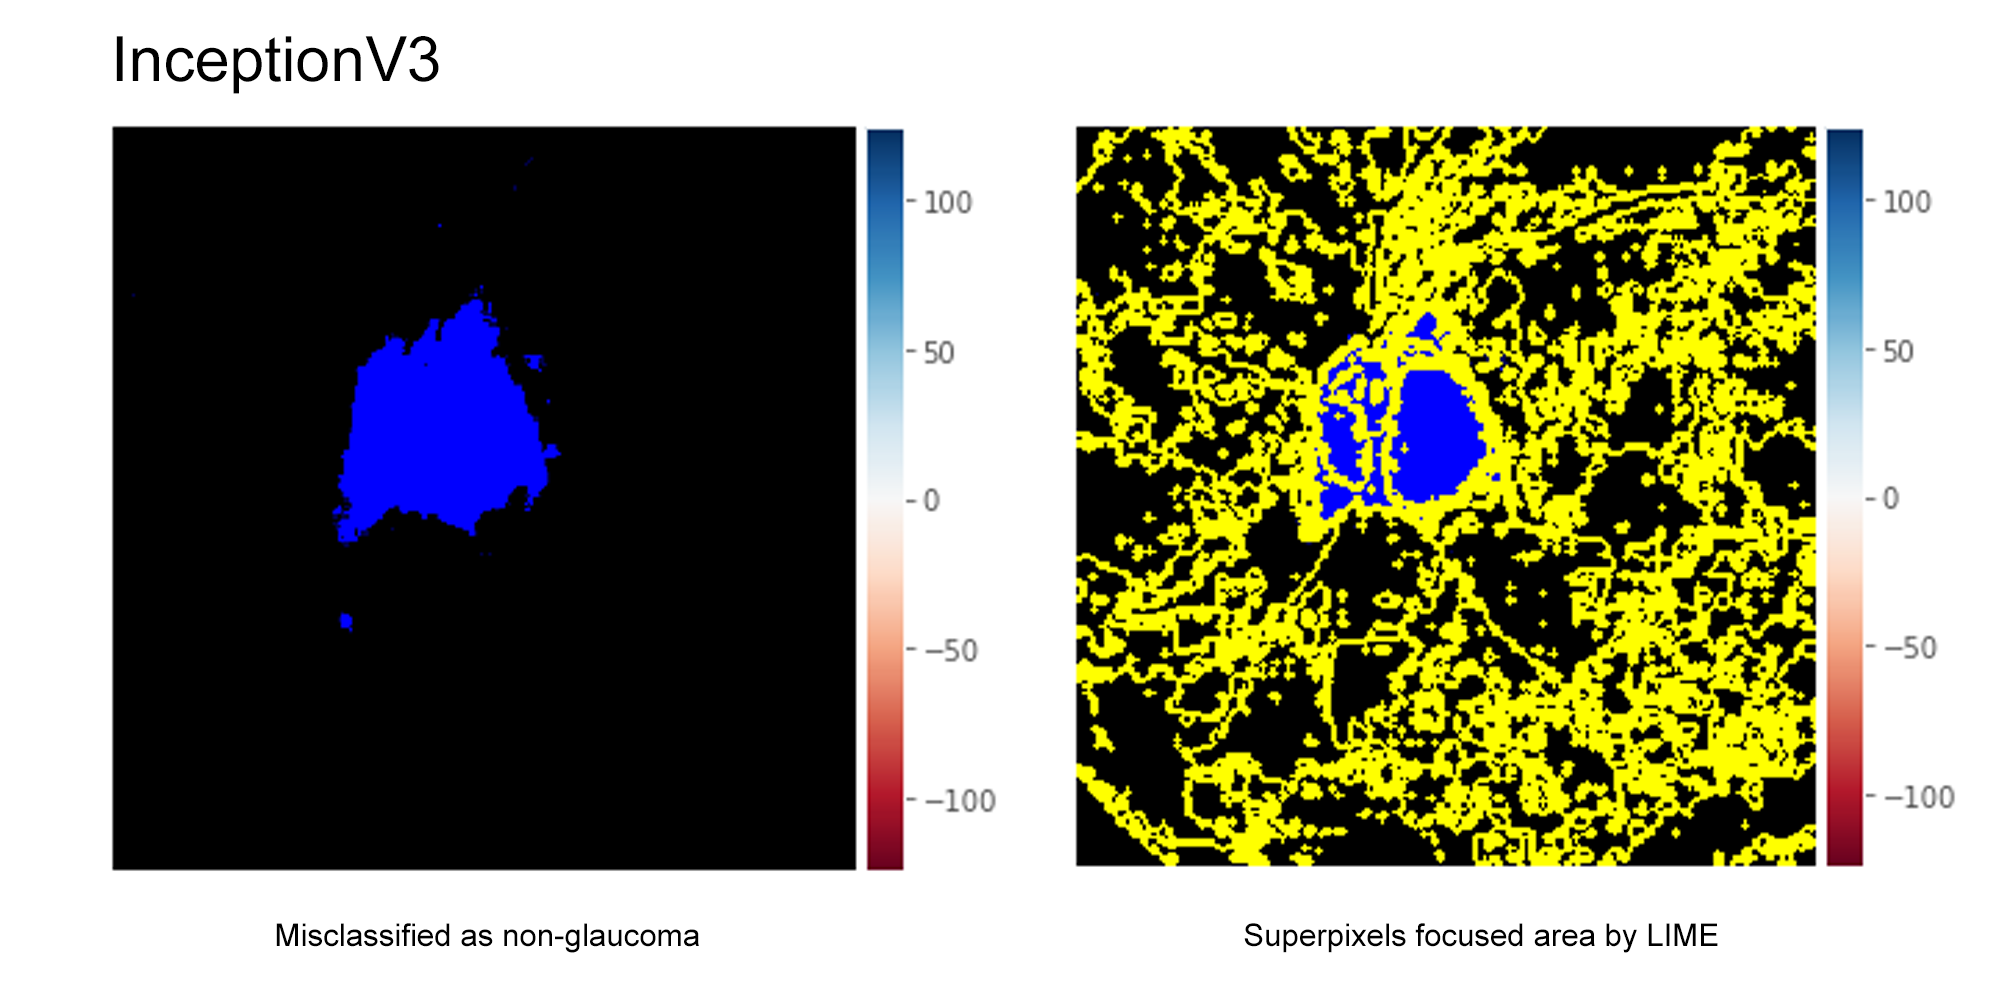
\includegraphics[scale=0.45]{images/fig-44.png}
\caption{Misclassified image with preprocessing and Superpixels focused area by Lime in InceptionV3
}
\label{fig:x Misclassified image with preprocessing and Superpixels focused area by Lime in InceptionV3
}
\end{figure}

\vspace{5mm}
\begin{figure}[hbt!]
\centering
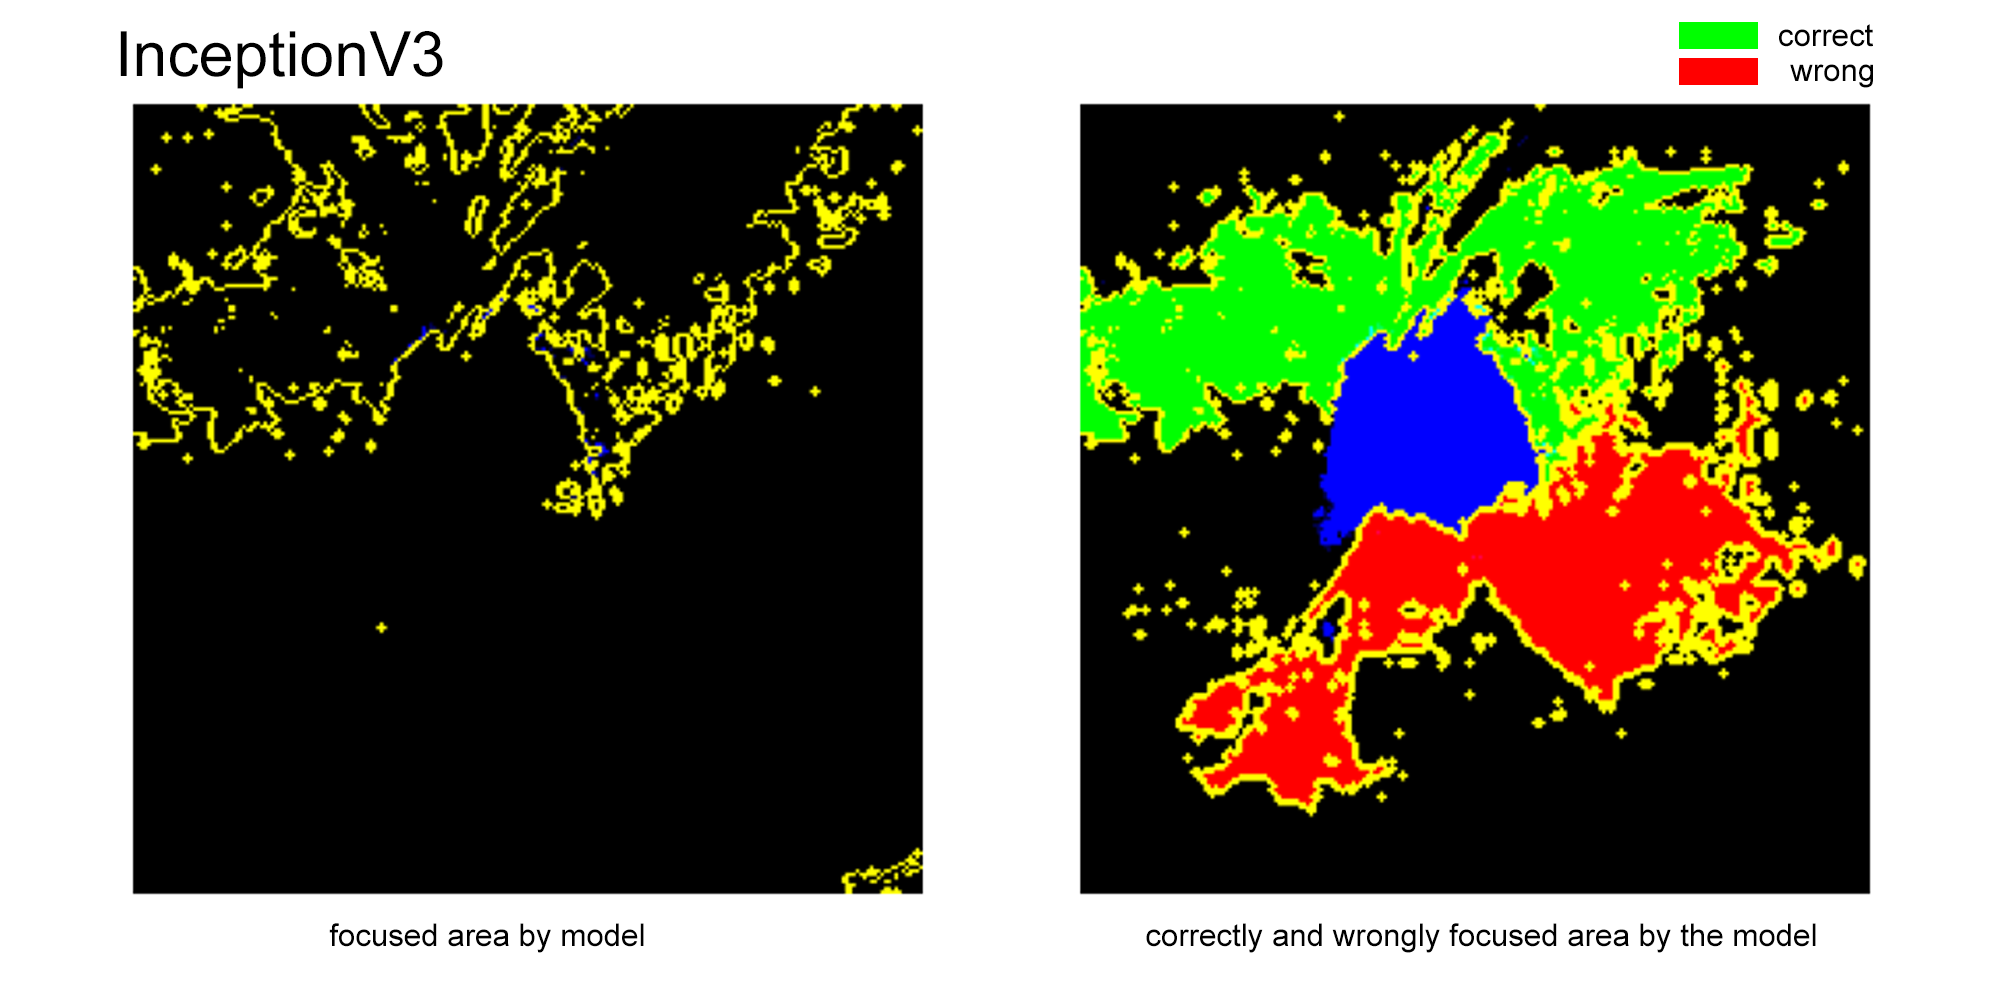
\includegraphics[scale=0.45]{images/fig-45.png}
\caption{Lime Explanation for InceptionV3}
\label{fig:x Lime Explanation for InceptionV3}
\end{figure}

\newpage
\vspace{5mm}
\noindent Given below are the the misclassified image with preprocessing, Superpixels focused area and the model prediction explanation by Lime in VGG-16 -

\vspace{5mm}
\begin{figure}[hbt!]
\centering
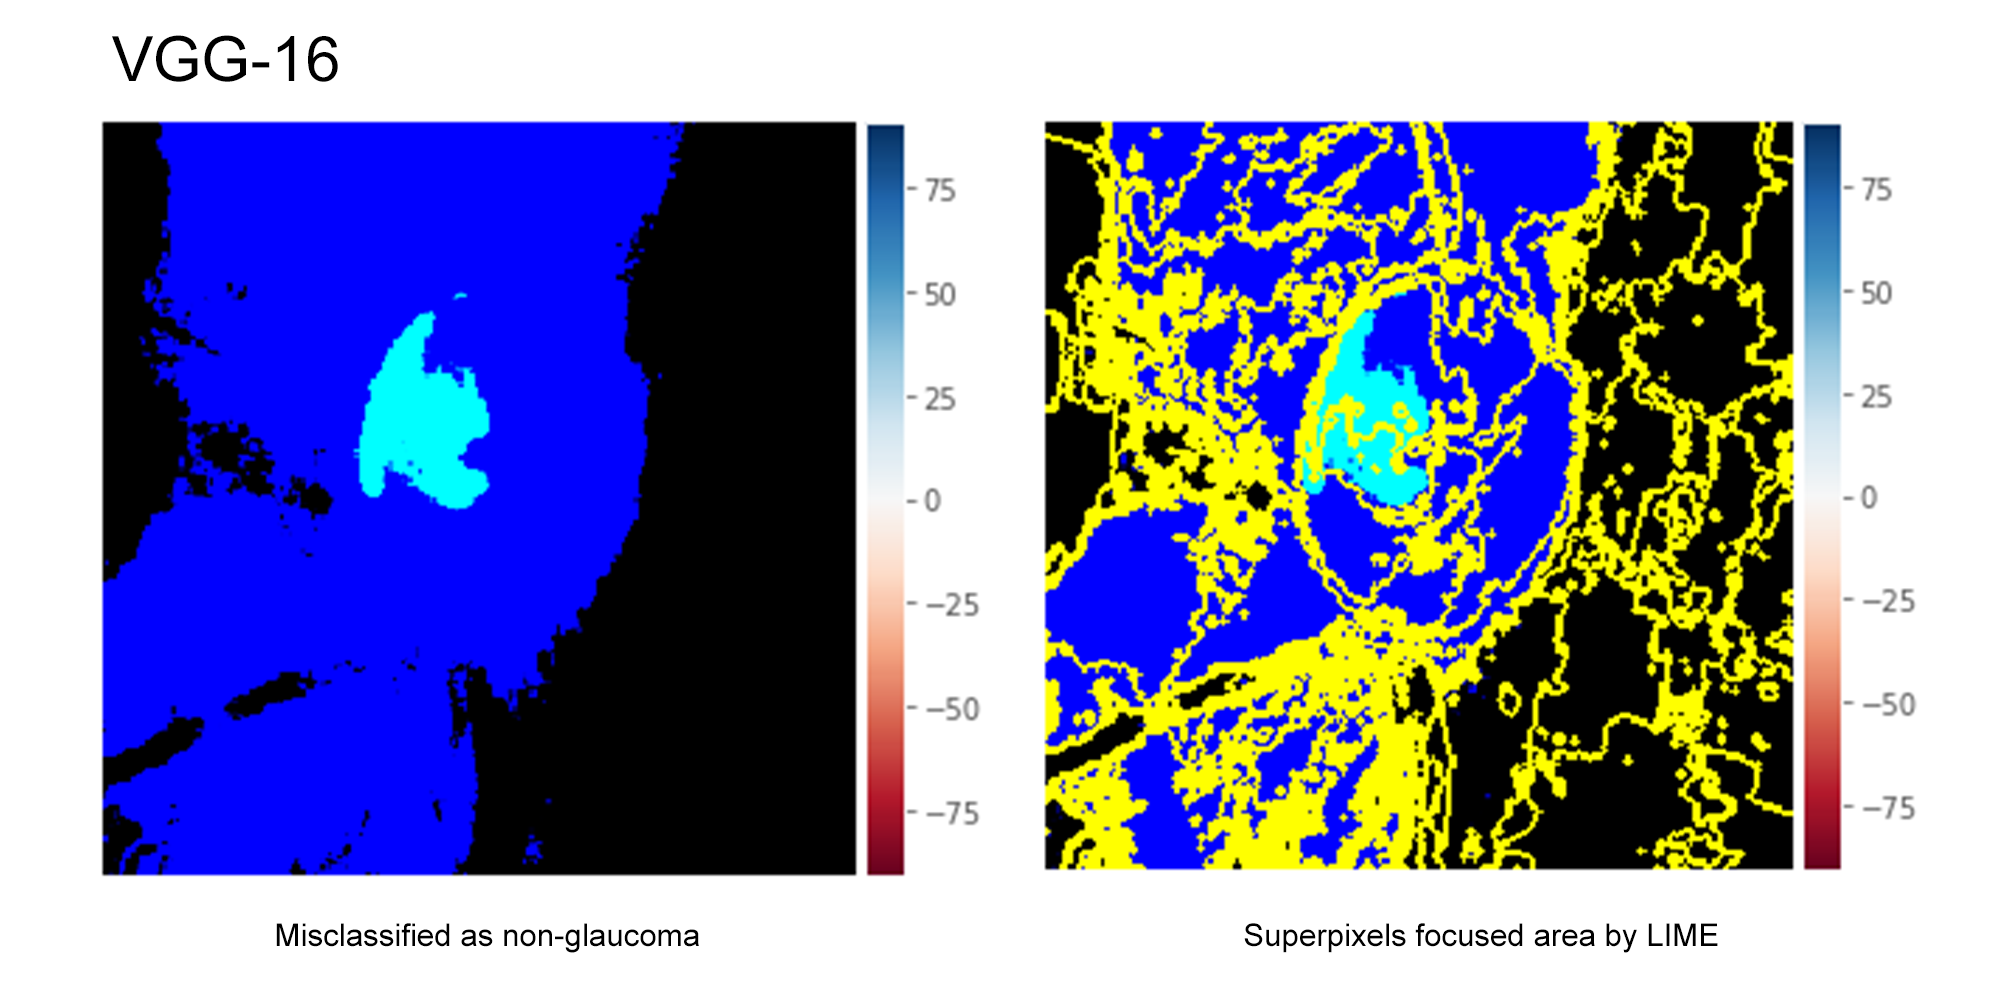
\includegraphics[scale=0.45]{images/fig-46.png}
\caption{Misclassified image with preprocessing and Superpixels focused area by Lime in VGG-16}
\label{fig:x Misclassified image with preprocessing and Superpixels focused area by Lime in VGG-16}
\end{figure}

\vspace{5mm}
\begin{figure}[hbt!]
\centering
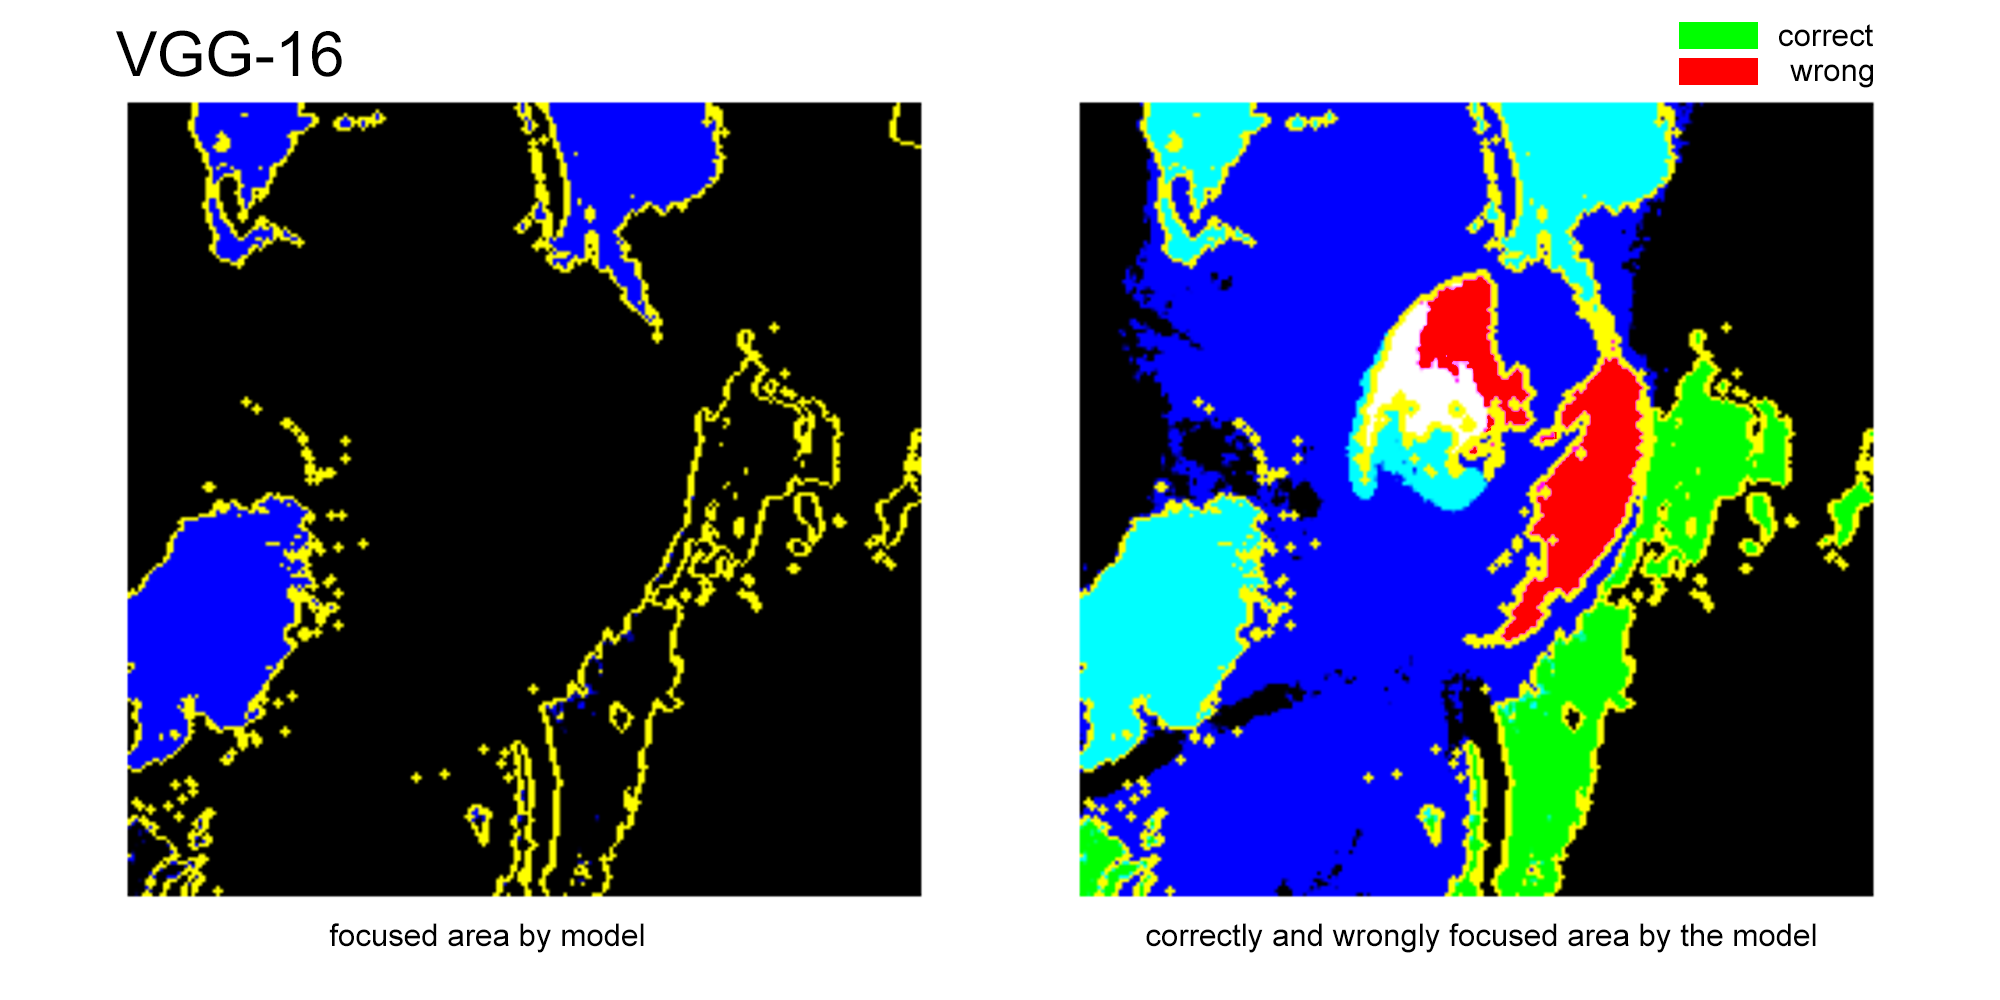
\includegraphics[scale=0.45]{images/fig-47.png}
\caption{Lime Explanation for VGG-16}
\label{fig:x Lime Explanation for VGG-16}
\end{figure}

\newpage
\vspace{5mm}
\noindent Given below are the the misclassified image with preprocessing, Superpixels focused area and the model prediction explanation by Lime in VGG-19 -

\vspace{5mm}
\begin{figure}[hbt!]
\centering
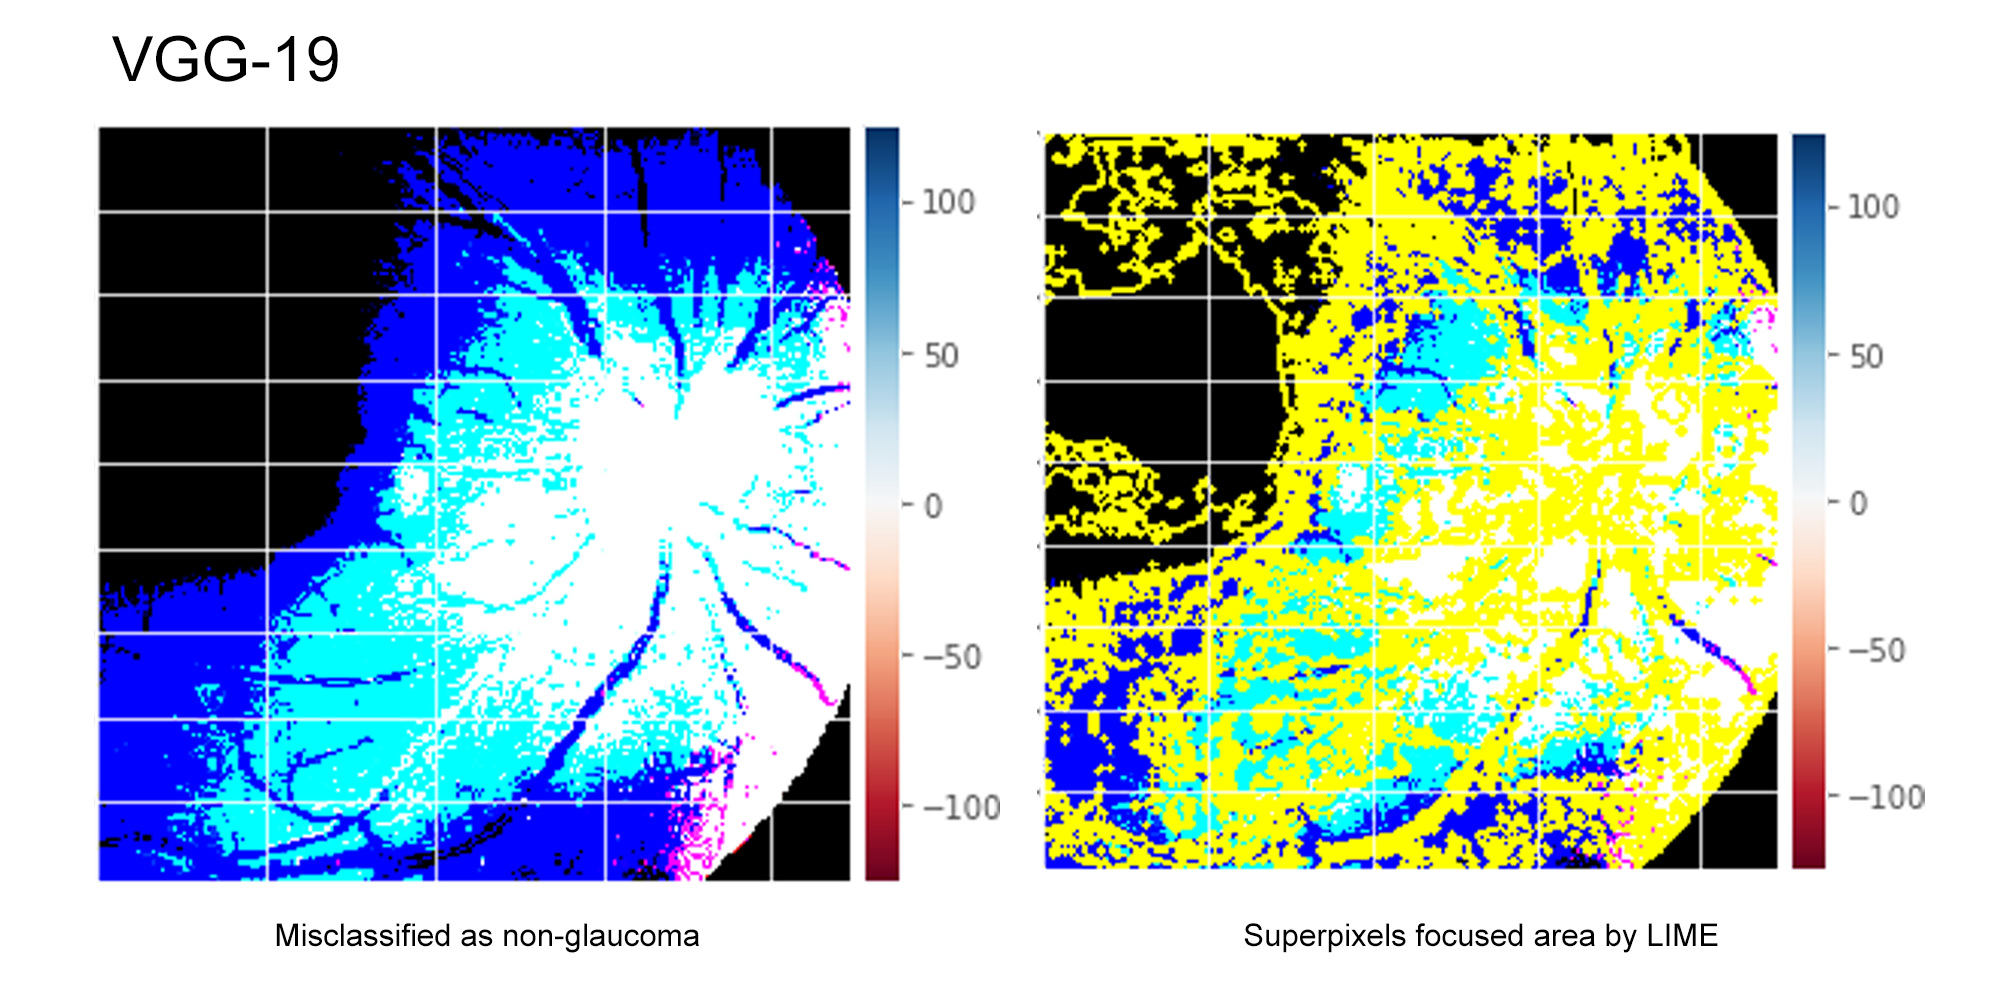
\includegraphics[scale=0.45]{images/fig-48.png}
\caption{Misclassified image with preprocessing and Superpixels focused area by Lime in VGG-19}
\label{fig:x Misclassified image with preprocessing and Superpixels focused area by Lime in VGG-19}
\end{figure}

\vspace{5mm}
\begin{figure}[hbt!]
\centering
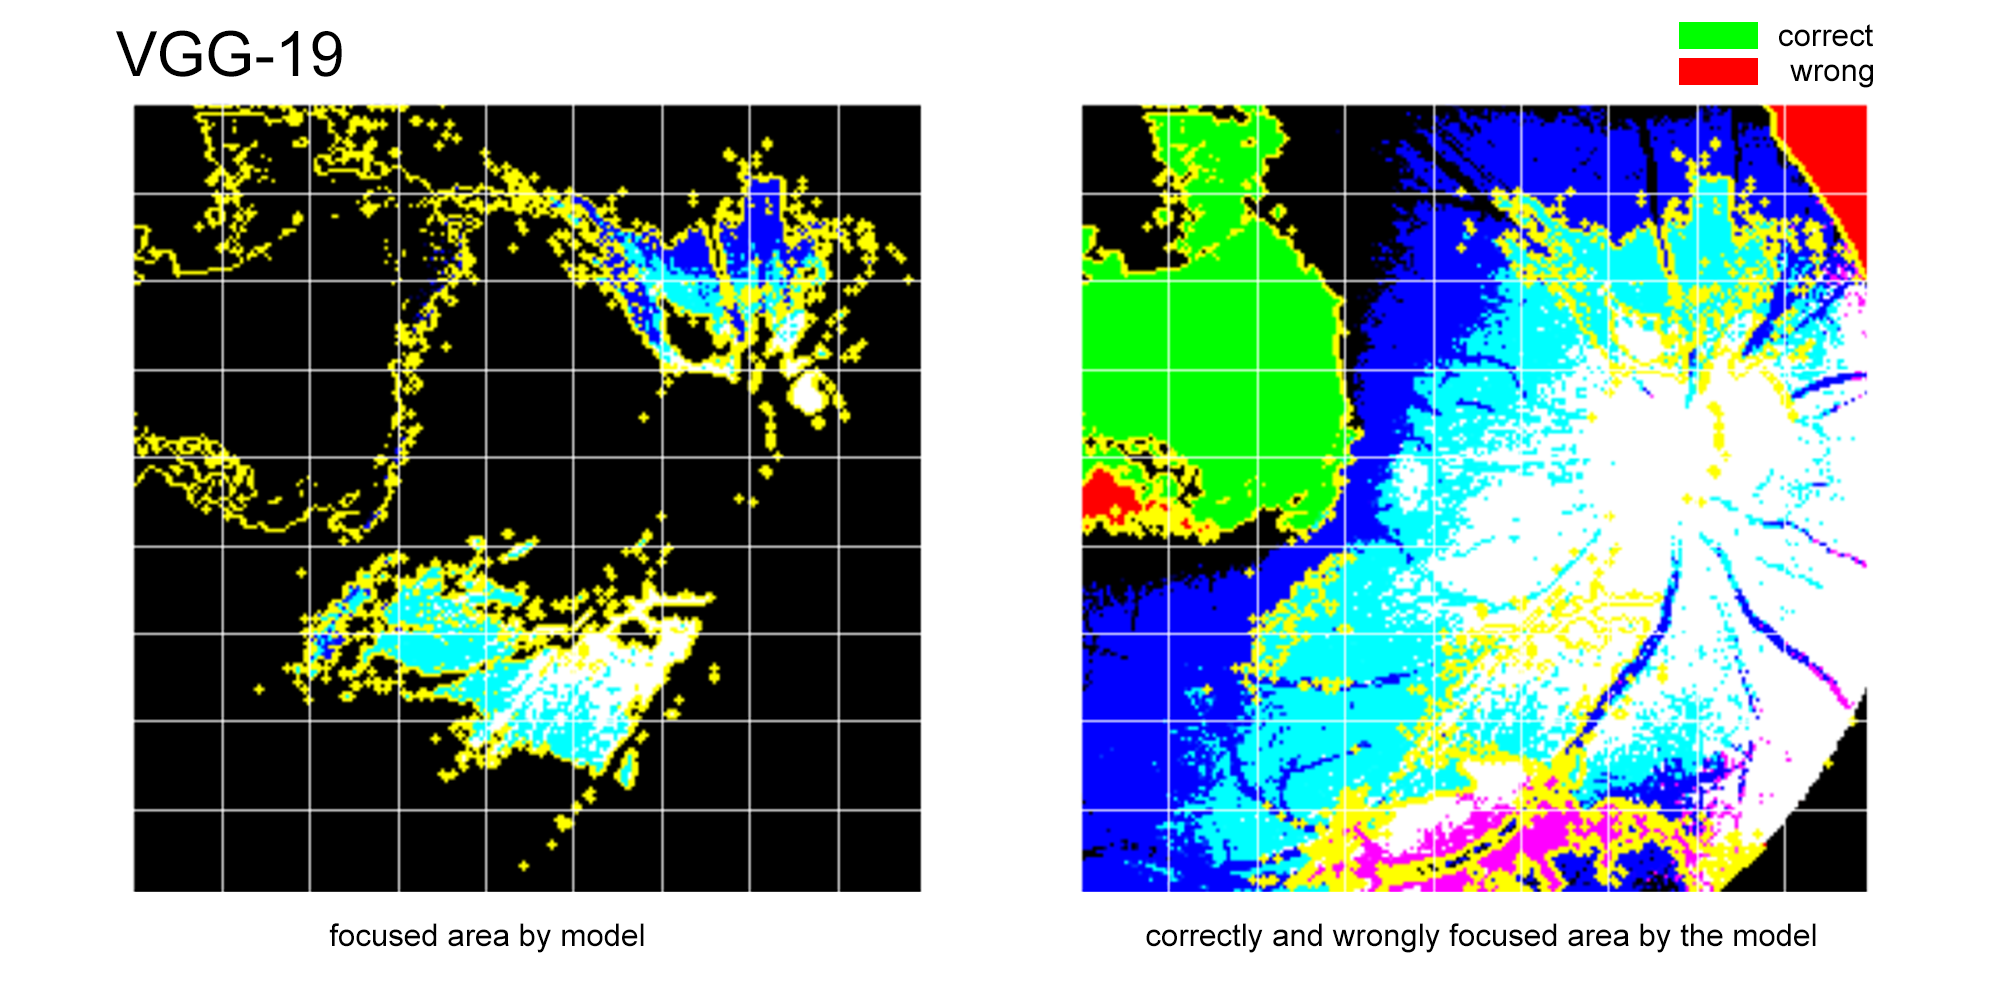
\includegraphics[scale=0.45]{images/fig-49.png}
\caption{Lime Explanation for VGG-19}
\label{fig:x Lime Explanation for VGG-19}
\end{figure}

\newpage
\vspace{5mm}
\noindent Given below are the the misclassified image with preprocessing, Superpixels focused area and the model prediction explanation by Lime in ResNet50 -

\vspace{5mm}
\begin{figure}[hbt!]
\centering
\includegraphics[scale=0.45]{images/fig-50.png}
\caption{Misclassified image with preprocessing and Superpixels focused area by Lime in ResNet50}
\label{fig:x Misclassified image with preprocessing and Superpixels focused area by Lime in ResNet50}
\end{figure}

\vspace{5mm}
\begin{figure}[hbt!]
\centering
\includegraphics[scale=0.45]{images/fig-51.png}
\caption{Lime Explanation for ResNet50}
\label{fig:x Lime Explanation for ResNet50}
\end{figure}

\newpage
\vspace{5mm}
Now for the single predicted raw fundus image -

\vspace{5mm}
\begin{figure}[hbt!]
\centering
\includegraphics[scale=0.20]{images/fig-52.png}
\caption{Lime Explanation for all models single image predictions}
\label{fig:x Lime Explanation for all models single image predictions}
\end{figure}

\newpage
\section{Result}
These are the single image predictions of all models - 

\noindent\textit{( here outputs are given in [n,m] format, where “m” means glaucoma score and “n” means non-glaucoma score )}

\vspace{5mm}
\begin{figure}[hbt!]
\centering
\includegraphics[scale=0.6]{images/fig-53.png}
\caption{Single Image Predictions for all Model}
\label{fig:x Single Image Predictions for all Model}
\end{figure}

\newpage
\vspace{5mm}
\noindent\textit{These are batch (50 images/batch) image predictions of all models - ( here [1,0] means glaucoma and [0,1] means non-glaucoma )}


\vspace{5mm}
\begin{figure}[hbt!]
\centering
\includegraphics[scale=0.6]{images/fig-54.png}
\caption{Batch Predictions for DenseNet121}
\label{fig:x Batch Predictions for DenseNet121}
\end{figure}

\vspace{5mm}
\begin{figure}[hbt!]
\centering
\includegraphics[scale=0.6]{images/fig-55.png}
\caption{Batch Predictions for InceptionV3}
\label{fig:x Batch Predictions for InceptionV3}
\end{figure}

\newpage
\vspace{5mm}
\noindent\textit{These are batch (50 images/batch) image predictions of all models - ( here [1,0] means glaucoma and [0,1] means non-glaucoma )}

\vspace{5mm}
\begin{figure}[hbt!]
\centering
\includegraphics[scale=0.6]{images/fig-56.png}
\caption{Batch Predictions for VGG-16}
\label{fig:x Batch Predictions for VGG-16}
\end{figure}

\vspace{5mm}
\begin{figure}[hbt!]
\centering
\includegraphics[scale=0.6]{images/fig-57.png}
\caption{Batch Predictions for VGG-19}
\label{fig:x Batch Predictions for VGG-19}
\end{figure}

\vspace{5mm}
\begin{figure}[hbt!]
\centering
\includegraphics[scale=0.6]{images/fig-58.png}
\caption{ Batch Predictions for ResNet50}
\label{fig:x  Batch Predictions for ResNet50}
\end{figure}



\nomenclature{$OOP$}{Object Oriented Programming}

\chapter{Conclusion}
%\section{Conclusion}
\section{Conclusion} 
In this research, to attain the ultimate objective of our study in Glaucoma Diagnosis, the Black
Box model was defined using Explainable Artificial Intelligence (XAI). As we have introduced
our work we have done so far in this research paper. Through this research, we were led to more
glaucoma diagnosis acceptability. Notably, glaucoma can take away the vision of a patient which
is why it’s more important to work for a better solution for early stage detection of glaucoma
disease. For this reason, using the XAI, recognition, and treatment of Glaucoma can bring an
immense change in the system which is very important, as reducing the number of blindness
caused by glaucoma through early proper detection and treatment of the disease is going to be a
huge success to celebrate. Because around the world 1 out of 15 people are blind because of it.
Statistics show that even with the treatment 15% to 20% of the patients become blind. To serve
our purpose we have used VGG-16, VGG-19, DenseNet121, InceptionV3 and ResNet50 models
for our study. Every model was compiled with Adam optimizer with the learning rate of 1e-5 in
50 epochs. If we look at the score which is validation accuracy for our models we can see that in
InceptionV3 we got 86.4\% accuracy, in DenseNet121 we got 86.8\% accuracy, in ResNet50 we
got 94.7\% accuracy, in VGG-19 we got 93.3\% accuracy and lastly in VGG-16 we got 88.6\%
accuracy. As the results showed, after 50 epochs, RestNet50 got the highest score among the
other models with a validation accuracy of 94.7\%. Afterwards we compared all models' accuracy
and loss graph together, where we can see that VGG-19 and ResNet50 were the Good-Fit than
the other models. So for our purpose we are proposing to use the LIME for getting rid of the very
lessened percentage in accuracy. Thereupon, in this research authors mentioned and showed how
they have used Deep Neural Network Leveraging Explainable Artificial Intelligence to reduce
the amount of Glaucoma Patients through early detection. Since there still is no known approach
to prevent glaucoma, glaucoma-related blindness or major visual loss can be avoided if the
condition is detected at an early stage. As now the AI has been improved and gained reliability in
the medical sector so as per research it can be prevented by early detection. To sum up, we can
say this research has achieved the goal to bring more accuracy, reliability and committed to
improving more in Glaucoma diagnosis to make a difference in human life and contribute
accordingly.

%\section{Bibliography}
\justifying
\section*{Bibliography} 
\noindent[1] Salam, A. A., Khalil, T., Akram, M. U., Jameel, A., & Basit, I. (2016). Automated detection of glaucoma using structural and non structural features. SpringerPlus, 5(1).\\ https://doi.org/10.1186/s40064-016-3175-4

\vspace{5mm}
\noindent[2] Ran, A., & Cheung, C. Y. (2021). Deep Learning-Based Optical Coherence Tomography and Optical Coherence Tomography Angiography Image Analysis: An Updated Summary. Asia-Pacific Journal of Ophthalmology, 10(3), 253–260. 

\noindent https://doi.org/10.1097/apo.0000000000000405

\vspace{5mm}
\noindent[3] Aleci, C. (2020). Detection of Visual Field Loss Progression in Glaucoma: An Overview and Food for Thought. Ophthalmology Research: An International Journal, 16–24.\\
https://doi.org/10.9734/or/2020/v13i130158

\vspace{5mm}
\noindent[4] Saha, S., Wang, Z., Sadda, S., Kanagasingam, Y., & Hu, Z. (2020). Visualizing and understanding inherent features in SD‐OCT for the progression of age‐related macular degeneration using deconvolutional neural networks. Applied AI Letters, 1(1). 

\noindent https://doi.org/10.1002/ail2.16
 
\vspace{5mm}
\noindent[5] Civit-Masot, J., Dominguez-Morales, M. J., Vicente-Diaz, S., & Civit, A. (2020). Dual Machine-Learning System to Aid Glaucoma Diagnosis Using Disc and Cup Feature Extraction. IEEE Access, 8, 127519–127529. 

\noindent https://doi.org/10.1109/access.2020.3008539

\vspace{5mm}
\noindent[6] Diabetic Retinopathy | National Eye Institute. (2021, July 30). National Eye Institute. 

\noindent https://www.nei.nih.gov/learn-about-eye-health/eye-conditions-and-diseases/diabetic-retinopathy

\vspace{5mm}
\noindent[7] Types of Glaucoma.(2020, June 2). Glaucoma Research Foundation. 

\noindent https://www.glaucoma.org/glaucoma/types-of-glaucoma.php#:\%7E:text=There\%20are\% 20several\%20types\%20of,or\%20pressure\%20inside\%20the\%20eye

\vspace{5mm}
\noindent[8] Saba, T., Khan, M. W., Yasmin, M., & Sharif, M. (2017). CDR based glaucoma detection using fundus images: a review. International Journal of Applied Pattern Recognition, 4(3), 261. 

\noindent https://doi.org/10.1504/ijapr.2017.10007613

\vspace{5mm}
\noindent[9] Thakoor, K. A., Li, X., Tsamis, E., Sajda, P., & Hood, D. C. (2019). Enhancing the Accuracy of Glaucoma Detection from OCT Probability Maps using Convolutional Neural Networks. 2019 41st Annual International Conference of the IEEE Engineering in Medicine and Biology Society (EMBC). 

\noindent https://doi.org/10.1109/embc.2019.8856899

\vspace{5mm}
\noindent[10]  Lim, T. C., Chattopadhyay, S., & Acharya, U. R. (2012). A survey and comparative study on the instruments for glaucoma detection. Medical Engineering & Physics, 34(2), 129–139. 

\noindent https://doi.org/10.1016/j.medengphy.2011.07.030

\vspace{5mm}
\noindent[11] Muddamsetty, S. M., Jahromi, M. N. S., & Moeslund, T. B. (2021b). Expert Level Evaluations for Explainable AI (XAI) Methods in the Medical Domain. Pattern Recognition. ICPR International Workshops and Challenges, 35–46. 

\noindent https://doi.org/10.1007/978-3-030-68796-0_3

\vspace{5mm}
\noindent[12] Abbas, Q. (2017). Glaucoma-Deep: Detection of Glaucoma Eye Disease on Retinal Fundus Images using Deep Learning. International Journal of Advanced Computer Science and Applications, 8(6). 

\noindent https://doi.org/10.14569/ijacsa.2017.080606

\vspace{5mm}
\noindent[13]  Dervisevic, E., Pavljasevic, S., Dervisevic, A., & Kasumovic, A. (2016). Challenges In Early Glaucoma Detection. Medical Archives, 70(3), 203. 

\noindent https://doi.org/10.5455/medarh.2016.70.203-207

\vspace{5mm}
\noindent[14]  R. Asaoka, H. Murata, A. Iwase, M. Araie, “Detecting preperimetric Glaucoma with Standard Automated Perimetry Using a Deep Learning Classifier,” Ophthalmology, vol. 123, pp. 1974–1980, September 2016.

\vspace{5mm}
\noindent[15]  Mayro, E.L., Wang, M., Elze, T. et al. The impact of artificial intelligence in the diagnosis and management of glaucoma. Eye 34, 1–11 (2020). 

\noindent https://doi.org/10.1016/j.ophtha.2016.05.029

\vspace{5mm}
\noindent[16]  Shabbir, A., Rasheed, A., Shehraz, H., Saleem, A., Zafar, B., Sajid, M., Ali, N., Dar, S. H., & Shehryar, T. (2021). Detection of glaucoma using retinal fundus images: A comprehensive review. Mathematical Biosciences and Engineering, 18(3), 2033–2076. 

\noindent https://doi.org/10.3934/mbe.2021106

\vspace{5mm}
\noindent[17] Brown, J. M., & Leontidis, G. (2021). Deep learning for computer-aided diagnosis in ophthalmology: a review. State of the Art in Neural Networks and their Applications, 219-237.


\noindent https://www.sciencedirect.com/science/article/pii/B9780128197400000115

\vspace{5mm}
\noindent[18] Sau, P. C., Gupta, M., & Kumar, D. (2021). A Comparative Study: Glaucoma Detection Using Deep Neural Networks. In Proceedings of International Conference on Big Data, Machine Learning and their Applications (pp. 85-97). Springer, Singapore.

\noindent https://link.springer.com/chapter/10.1007/978-981-15-8377-3_8

\vspace{5mm}
\noindent[19] Greco, A., Rizzo, M. I., De Virgilio, A., Gallo, A., Fusconi, M., de Vincentiis, M. (2016). Emerging concepts in Glaucoma and review of the literature. The American Journal of Medicine (2016).

\noindent https://doi.org/10.1016/j.amjmed.2016.03.038

\vspace{5mm}
\noindent[20] Pascolini, D., & Mariotti, S. P. (2012). Global estimates of visual impairment: 2010. British Journal of Ophthalmology, 96(5), 614-618.

\noindent https://bjo.bmj.com/content/96/5/614.short

\vspace{5mm}
\noindent[21] Goldbaum MH, Sample PA, White H, Colt B, Raphaelian P, Fechtner RD, et al. Interpretation of automated perimetry for glaucoma by neural network. Invest Ophthalmol Vis Sci. 1994;35:3362–73. 


\noindent\url{https://www.researchgate.net/publication/15141759_Interpretation_of_automated\\_perimetry_for_glaucoma_by_neural_network}

\vspace{5mm}
\noindent[22]  Murphy, A. M., & Moore, C. M. M. (2020). Fully connected neural network. 

\noindent https://radiopaedia.org/articles/fully-connected-neural-network

\vspace{5mm}
\noindent[23] Brownlee, J. (2020, August 14). What is Deep Learning? Machine Learning Mastery. 

\noindent https://machinelearningmastery.com/what-is-deep-learning/

\vspace{5mm}
\noindent[24] Khan, S. M. K. (2021, January 3). Papers with Code - LAG Dataset. The Lancet. 

\noindent https://paperswithcode.com/dataset/lag

\vspace{5mm}
\noindent[25] How to fine-tune your artificial intelligence algorithms 

\noindent https://www.allerin.com/blog/how-to-fine-tune-your-artificial-intelligence-algorithms

\vspace{5mm}
\noindent[26] Saxena, A., Vyas, A., Parashar, L., & Singh, U. (2020, July). A glaucoma detection using a convolutional neural network. In 2020 International Conference on Electronics and Sustainable Communication Systems (ICESC) (pp. 815-820). IEEE.

\noindent https://ieeexplore.ieee.org/abstract/document/9155930/

\vspace{5mm}
\noindent[27] Dervisevic, E., Pavljasevic, S., Dervisevic, A., & Kasumovic, S. S. (2016). Challenges In Early Glaucoma Detection. Medical archives (Sarajevo, Bosnia and Herzegovina), 70(3), 203–207. 

\noindent https://doi.org/10.5455/medarh.2016.70.203-207

\vspace{5mm}
\noindent[28] Mash, Robert & Becherer, Nicholas & Woolley, Brian & Pecarina, John. (2016). Toward aircraft recognition with convolutional neural networks. 

\noindent https://doi.org/10.1109/NAECON.2016.7856803.

\vspace{5mm}
\noindent[29] Guo, T., Dong, J., Li, H., & Gao, Y. (2017). Simple convolutional neural network on image classification. 2017 IEEE 2nd International Conference on Big Data Analysis (ICBDA). 

\noindent https://doi.org/10.1109/icbda.2017.8078730

\vspace{5mm}
\noindent[30] Yamashita, R., Nishio, M., Do, R. K. G., & Togashi, K. (2018). Convolutional neural networks: an overview and application in radiology. Insights into Imaging, 9(4), 611–629. 

\noindent https://doi.org/10.1007/s13244-018-0639-9

\vspace{5mm}
\noindent[31] Yun-Cheng Tsai Predict Forex Trend via Convolutional Neural Networks 

\noindent https://www.degruyter.com/document/doi/10.1515/jisys-2018-0074/html

\vspace{5mm}
\noindent[32] Kaushik, A. (2020, February 26). Understanding the VGG19 Architecture. OpenGenus IQ: Computing Expertise & Legacy. 

\noindent\url{https://iq.opengenus.org/vgg19-architecture/#:\%7E:text=VGG19\%20is\%20a\%20variant\%20of,VGG19\%20has\%2019.6\%20billion\%20FLOPs.}

\vspace{5mm}
\noindent[33] Huang, G. (2016, August 25). Densely Connected Convolutional Networks. ArXiv.Org. 

\noindent https://arxiv.org/abs/1608.06993

\vspace{5mm}
\noindent[34] S. Saha, A comprehensive guide to convolutional neural networks — the eli5
way, Available at 

\noindent https://towardsdatascience.com/a-comprehensive-guide-toconvolutional-neural-networks-the-eli5-way-3bd2b1164a53, 2018. 

\vspace{5mm}
\noindent [35] Jeong, J. (2021, December 7). The Most Intuitive and Easiest Guide for Convolutional Neural Network. Medium. \\
\enablehyph{https://towardsdatascience.com/the-most-intuitive-and-easiest-guide-for-convolutional-neural-network-3607be47480}



\vspace{5mm}
\noindent[36] Singh, S. P. (2019, March 2). Fully Connected Layer: The brute force layer of a Machine Learning model. OpenGenus IQ: Computing Expertise & Legacy. 

\noindent https://iq.opengenus.org/fully-connected-layer/

\vspace{5mm}
\noindent[37] Sergey Ioffe, Christian Szegedy.(2015). Batch Normalization: Accelerating Deep Network Training b y Reducing Internal Covariate Shift. 

\noindent https://arxiv.org/pdf/1502.03167.pdf
 
\vspace{5mm} 
\noindent[38] S. Wager, S. Wang, and P. S. Liang, training as adaptive regularization”, in Advances in Neural Information Processing Systems 26, C. J. C. Burges, L. Bottou, M. Welling, Z. Ghahramani, and K. Q. Weinberger, Eds., Curran Associates, Inc., 2013, pp. 351-359. [Online].  

\noindent http://papers. nips.cc/paper/4882-dropout-training-as-adaptive-regularization.pdf.

\vspace{5mm}
\noindent[39] Springenberg, J. T. (2014, December 21). Striving for Simplicity: The All Convolutional Net. ArXiv.Org. https://arxiv.org/abs/1412.6806

\vspace{5mm}
\noindent[40] Dağlarli, E. (2020). Explainable Artificial Intelligence (XAI) Approaches and Deep Meta-Learning Models. Advances and Applications in Deep Learning, 79. 

\noindent https://www.intechopen.com/chapters/72398

\vspace{5mm}
\noindent[41] Shabbir, A., Rasheed, A., Shehraz, H., Saleem, A., Zafar, B., Sajid, M., ... & Shehryar, T. (2021). Detection of glaucoma using retinal fundus images: A comprehensive review. Mathematical Biosciences and Engineering, 18(3), 2033-2076. 

\noindent http://aimspress.com/article/doi/10.3934/mbe.2021106

\vspace{5mm}
\noindent[42] Vejjanugraha, P., Kongprawechnon, W., Kondo, T., Tungpimolrut, K., & Kotani, K. (2017). An automatic screening method for primary open-angle glaucoma assessment using binary and multi-class support vector machines. ScienceAsia, 43(4), 229. 

\noindent https://doi.org/10.2306/scienceasia1513-1874.2017.43.229

\phantomsection
\printbibliography % Where the bibliography will be printed
\addcontentsline{toc}{chapter}{Bibliography}

% ********************************** Appendices ********************************
%\begin{appendices} % Using appendices environment for more functionality
% \newpage
% \phantomsection
% \addcontentsline{toc}{chapter}{Appendix A How to install \LaTeX}
% % ******************************* Thesis Appendix A ****************************
\chapter*{How to install \LaTeX} 

\section*{Windows OS}

\subsection*{TeXLive package - full version}
\begin{enumerate}
\item	Download the TeXLive ISO (2.2GB) from\\
\href{https://www.tug.org/texlive/}{https://www.tug.org/texlive/}
\item	Download WinCDEmu (if you don't have a virtual drive) from \\
\href{http://wincdemu.sysprogs.org/download/}
{http://wincdemu.sysprogs.org/download/}
\item	To install Windows CD Emulator follow the instructions at\\
\href{http://wincdemu.sysprogs.org/tutorials/install/}
{http://wincdemu.sysprogs.org/tutorials/install/}
\item	Right click the iso and mount it using the WinCDEmu as shown in \\
\href{http://wincdemu.sysprogs.org/tutorials/mount/}{
http://wincdemu.sysprogs.org/tutorials/mount/}
\item	Open your virtual drive and run setup.pl
\end{enumerate}

or

\subsection*{Basic MikTeX - \TeX~ distribution}
\begin{enumerate}
\item	Download Basic-MiK\TeX (32bit or 64bit) from\\
\href{http://miktex.org/download}{http://miktex.org/download}
\item	Run the installer 
\item	To add a new package go to Start >> All Programs >> MikTex >> Maintenance (Admin) and choose Package Manager
\item	Select or search for packages to install
\end{enumerate}

\subsection*{TexStudio - \TeX~ editor}
\begin{enumerate}
\item	Download TexStudio from\\
\href{http://texstudio.sourceforge.net/\#downloads}
{http://texstudio.sourceforge.net/\#downloads} 
\item	Run the installer
\end{enumerate}

\section*{Mac OS X}
\subsection*{MacTeX - \TeX~ distribution}
\begin{enumerate}
\item	Download the file from\\
\href{https://www.tug.org/mactex/}{https://www.tug.org/mactex/}
\item	Extract and double click to run the installer. It does the entire configuration, sit back and relax.
\end{enumerate}

\subsection*{TexStudio - \TeX~ editor}
\begin{enumerate}
\item	Download TexStudio from\\
\href{http://texstudio.sourceforge.net/\#downloads}
{http://texstudio.sourceforge.net/\#downloads} 
\item	Extract and Start
\end{enumerate}


\section*{Unix/Linux}
\subsection*{TeXLive - \TeX~ distribution}
\subsubsection*{Getting the distribution:}
\begin{enumerate}
\item	TexLive can be downloaded from\\
\href{http://www.tug.org/texlive/acquire-netinstall.html}
{http://www.tug.org/texlive/acquire-netinstall.html}.
\item	TexLive is provided by most operating system you can use (rpm,apt-get or yum) to get TexLive distributions
\end{enumerate}

\subsubsection*{Installation}
\begin{enumerate}
\item	Mount the ISO file in the mnt directory
\begin{verbatim}
mount -t iso9660 -o ro,loop,noauto /your/texlive####.iso /mnt
\end{verbatim}

\item	Install wget on your OS (use rpm, apt-get or yum install)
\item	Run the installer script install-tl.
\begin{verbatim}
	cd /your/download/directory
	./install-tl
\end{verbatim}
\item	Enter command `i' for installation

\item	Post-Installation configuration:\\
\href{http://www.tug.org/texlive/doc/texlive-en/texlive-en.html\#x1-320003.4.1}
{http://www.tug.org/texlive/doc/texlive-en/texlive-en.html\#x1-320003.4.1} 
\item	Set the path for the directory of TexLive binaries in your .bashrc file
\end{enumerate}

\subsubsection*{For 32bit OS}
For Bourne-compatible shells such as bash, and using Intel x86 GNU/Linux and a default directory setup as an example, the file to edit might be \begin{verbatim}
edit $~/.bashrc file and add following lines
PATH=/usr/local/texlive/2011/bin/i386-linux:$PATH; 
export PATH 
MANPATH=/usr/local/texlive/2011/texmf/doc/man:$MANPATH;
export MANPATH 
INFOPATH=/usr/local/texlive/2011/texmf/doc/info:$INFOPATH;
export INFOPATH
\end{verbatim}
\subsubsection*{For 64bit OS}
\begin{verbatim}
edit $~/.bashrc file and add following lines
PATH=/usr/local/texlive/2011/bin/x86_64-linux:$PATH;
export PATH 
MANPATH=/usr/local/texlive/2011/texmf/doc/man:$MANPATH;
export MANPATH 
INFOPATH=/usr/local/texlive/2011/texmf/doc/info:$INFOPATH;
export INFOPATH

\end{verbatim}



%\subsection{Installing directly using Linux packages} 
\subsubsection*{Fedora/RedHat/CentOS:}
\begin{verbatim} 
sudo yum install texlive 
sudo yum install psutils 
\end{verbatim}


\subsubsection*{SUSE:}
\begin{verbatim}
sudo zypper install texlive
\end{verbatim}


\subsubsection*{Debian/Ubuntu:}
\begin{verbatim} 
sudo apt-get install texlive texlive-latex-extra 
sudo apt-get install psutils
\end{verbatim}


% \newpage
% \phantomsection
% \addcontentsline{toc}{chapter}{Appendix B Overleaf: GitHub for \LaTeX\ projects}
% % ******************************* Thesis Appendix B ********************************

\chapter*{Overleaf: GitHub for \LaTeX\ projects }

This Project was developed using Overleaf(\url{https://www.overleaf.com/}), an online \LaTeX\ editor that allows real-time collaboration and online compiling of projects to PDF format. In comparison to other \LaTeX\ editors, Overleaf is a server-based application, which is accessed through a web browser.




%\end{appendices}

\end{document}